\documentclass[a4paper]{article}
\usepackage[latin1]{inputenc}
\usepackage[T1]{fontenc}
\usepackage{amsmath, amssymb}
\usepackage{amsthm}
\usepackage{lipsum}
\usepackage{float}
\usepackage{url}
\usepackage{graphicx}
\usepackage{subfig}
\usepackage{latexsym}
\usepackage{listings}
\usepackage[usenames]{color}
\usepackage{titling}
\usepackage{multirow}
\usepackage{chngpage}
\usepackage{adjustbox}
\usepackage[]{algorithm2e}

\SetKwRepeat{Do}{do}{while}

\definecolor{mygreen}{rgb}{0,0.6,0}
\definecolor{mygray}{rgb}{0.5,0.5,0.5}
\definecolor{myblue}{rgb}{0,0.1,0.7}
\definecolor{myyellow}{rgb}{1,1,0.6}
\definecolor{Red}{rgb}{1,0,0}
\definecolor{Green}{rgb}{0,0.6,0}

\lstdefinestyle{C}
{%basicstyle=\footnotesize,
basicstyle=\ttfamily,
keywordstyle=\color{myblue}\bfseries,
identifierstyle=\color{black},
commentstyle=\color{mygray}\itshape,
stringstyle=\color{Green}\ttfamily,
showstringspaces=false,
%numbers=left, numberstyle=\tiny,
%stepnumber=1, numbersep=5pt,
tabsize=4,
framexleftmargin=5mm, 
rulesepcolor=\color{mygray},
%frame=LtBr,
language={C},
fontadjust=true,
breaklines=true,
breakatwhitespace=true,
breakautoindent
}	

\setcounter{secnumdepth}{2}

\begin{document}

\begin{titlepage}
	\centering
	{\scshape\LARGE Universit� Degli Studi Di Padova \par}
	{\Large Course in Operations Research 2\par}
	\vspace{1.5cm}
	{\huge\bfseries Wind Farm Cables Routing Optimization\par}
	\vspace{2cm}
	{\Large\itshape Massimo Meneghello and Andrea Tommasi\par}
	\vspace{1.5cm}
	 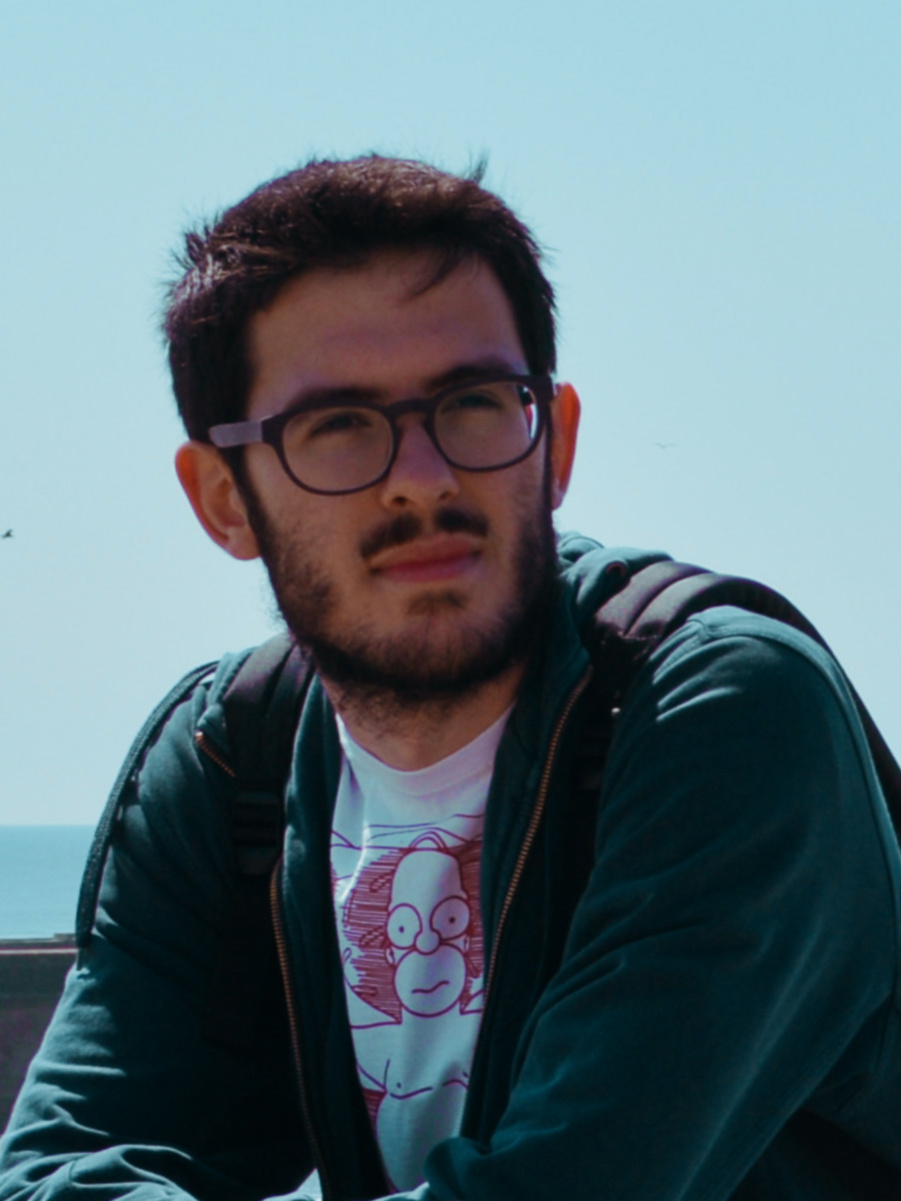
\includegraphics[scale=.1465]{img/massimo}
	 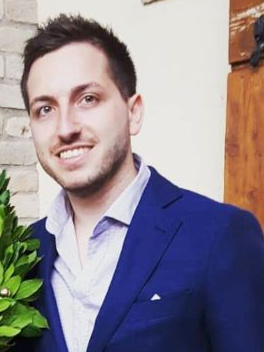
\includegraphics[scale=.50]{img/andrea}
	\vfill

% Bottom of the page
	{\large \today\par}
\end{titlepage}

%\maketitle

\newpage
\tableofcontents
\newpage

% DA RIVEDERE FINITA LA CORREZIONE
\section{Introduction}

Wind energy is a source of renewable power that comes from air currents flowing across the earth's surface.
Nowadays it is one of the new fastest growing sources of electricity in the world.
As the number of turbines per wind farm increases, it becomes extremely important to optimize the cable connections among them: on one hand, to lower installation costs, on the other, to reduce energy losses during operation.

In this paper, we first present a Mixed Integer Linear Programming (MILP) model that is able to handle most of the required real-world constraints.
Subsequently, we show several optimization approaches to solve this problem, and we report the collected data on different existing wind farms.

For a more exhaustive account on wind farm optimization, see \cite{FISCHETTI2018917}: we used this article as a benchmark for our work, developing the same mathematical model and using the same test bed in order to compare the results.\\

In chapter \ref{sec:MILPModel}, we present a comprehensive description of the mathematical model we used, providing details regarding peculiar constraints and relaxed versions of the model.

Chapter \ref{sec:implementingAndSolvingWithCPLEX} focuses on solving the MILP model.
In the first part, we present a brief introduction to the \texttt{CPLEX} optimization software and we show how to use its main features, in particular, the \emph{lazy constraints} and the \emph{callbacks}. 
Then, we provide a solution that uses \texttt{CPLEX} as a \emph{black box}, called the \emph{Loop Method}.

In chapter \ref{sec:HeuristicSolvers}, we show a matheuristic strategy, the \emph{Hard-fixing} and two heuristic approaches we entirely designed and coded.
In this case, we decided to use a \emph{multi-start} (MS) approach and the \emph{Variable Neighborhood Search} (VNS) heuristics.

Finally, chapter \ref{sec:results} contains information about the results we collected in our experiments and the main differences with respect to the results Fischetti and Pisinger reported in their work \cite{FISCHETTI2018917}.

\newpage

% CORRETTO TUTTO
\section{MILP Model}
\label{sec:MILPModel}

In each offshore wind farm, one or more substations collect all the power of the turbines and convey this energy to the mainland.
Each turbine must be joined through a cable to another turbine or to a substation.
The final layout can be represented with a \emph{tree} structure (or a \emph{forest}, in presence of many substations), where all the nodes are connected to one substation (the root of the tree). This layout is called \emph{cables routing}.

In this article, we do not take into account the problem of positioning the turbines.
In fact, we only analyze real instances in which the turbines have already been placed.
A specific description of this subject is instead provided in \cite{10.1007/978-4-431-55420-2_4}.

Additionally, in order to simplify the representation of the problem, all examples we consider in this report involve only one substation.

Therefore, assuming that the best turbine positions have been identified, we aim at finding an optimal cables routing among all the turbines and the substation, minimizing the total cables amount.

\subsection{Basic Model}

In the mathematical model in \cite{FISCHETTI2018917}, the following constraints are taken into account.

The first constraint to satisfy is the balance of flows: the energy flow entering a turbine must be equivalent to the outgoing one, plus the turbine's production.
Moreover, only one cable can come out of each turbine, so we must have a flow at most equal to the capacity of the biggest cable provided because every cable installed must withstand the power coming out of the turbine. 

Another limitation is the substation's capability, named the maximum number of cables that the substation can accept. In our testbed, the substation has a parameter, indicated as $C$, representing this value.

All the instances we consider are composed of a wind farm layout and a set of cables that can be used for the layout: each cable presents a different cost and capacity.
In the following, we say $n$ to be the number of turbines (including the substation) in the layout and we indicate as $K$ the cardinality of the cables' set.

We can describe the cables routing as a direct graph $G = (V, A)$, with $V = \{1,\hdots,n\}$ representing the set of turbines and $A$ denoting the set of arcs.
We recall that in a direct graph $(i,j) \neq (j,i)$, while $\{i,j\}$ stands for $(i,j)$ and $(j,i)$.\\

Every arc must cope a \emph{flow} that represents the energy captured by the turbines in the subtree from which the arc is coming out. We represent the flow running from $i$ to $j$ with the variable
\begin{gather}
\label{eqn:fVariables}
f_{i,j} \ge 0, \; \forall\,(i,j) \in A.
\end{gather}

The second class of variables in our model indicates whether an arc $(i,j) \in A$ is build using a cable of type $k$:
\begin{equation}
\begin{gathered}
\label{eqn:xVariables}
x_{i,j}^k = 
		\begin{cases}
		1 \quad \text{if arc $(i,j) \in A$ is built with a cable of type $k$}\\
		0 \quad \text{otherwise.}
		\end{cases}\\	
		\forall\,(i,j) \in A, \forall\,k\,:\,1 \le k \le K
\end{gathered}
\end{equation}

Our last type of variables indicates whether an arc $(i,j)$ of $G$ is selected for the cables routing or not:
\begin{equation}
\begin{gathered}
\label{eqn:yVariables}
y_{i,j} = 
		\begin{cases}
		1 \quad \text{if arc $(i,j) \in A$ is selected for the cables routing}\\
		0 \quad \text{otherwise.}
		\end{cases}\\
		\forall\,(i,j) \in A
\end{gathered}
\end{equation}

Regarding the model's constraints, the first type of constraints is the one imposing that an arc $(i,j)$ can be built using just one type of cables.
\begin{gather}
\label{eqn:yConstraints}
y_{i,j} = \sum_{k=1}^K x_{i,j}^k, \quad \forall\,(i,j) \in A.
\end{gather}

Next, we add out-degree constraints for turbines and substation: we desire that only one cable comes out from each turbine. The $P_h$ value indicates the energy produced by the turbine $h$: if this value is equal to $-1$ means that $h$ is the substation and no cable must exit from it.
\begin{gather}
\label{eqn:outDegConstraints}
\sum_{j=1}^n y_{h,j} = 
		\begin{cases}
		1 \quad \text{if $P_h > 0 $} \\
		0 \quad \text{if $P_h = -1$ \quad (substation)}
		\end{cases} \forall\,h \in V
\end{gather}

With the subsequent, we want to pose a restriction to the number of cables entering the substation and we want this quantity to be less than or equal to parameter $C$:
\begin{gather}
\label{eqn:substationInDegConstraint}
\sum_{i=1}^n y_{i,h} \le C, \quad \forall\,h \in V : P_h = -1.
\end{gather}

In order to avoid self-loops, we also impose that
\begin{gather}
y_{i,i} = 0, \quad \forall\,i\in V
\end{gather}

Another significant rule to catch is the balance of flows: the flow entering a turbine must equal the outgoing one plus the power $P_h$ produced by the turbine $h$.
\begin{gather}
\label{eqn:flowsContraints}
\sum_{j=1}^n f_{h,j} = \sum_{i=1}^n f_{i,h} + P_h, \quad \forall\,h \in V : P_h \ge 0.
\end{gather}

The energy flow leaving a turbine must be supported by a single cable, consequently, the capacity of the cable from turbine $i$ to $j$ must be greater or equal to the flow $f_{i,j}$ coming out from turbine $i$. Saying $cap(k)$ be the maximum capacity of type k cable, this constraint can be expressed as:
\begin{gather}
\label{eqn:capacityConstraints}
\sum_{k=1}^K cap(k) \cdot x_{i,j}^k \ge f_{i,j}, \quad \forall\,(i,j) \in A.
\end{gather}

Finally, what we desire to minimize is the total amount of posed cables, considering as well the cost of the different types of them. Saying $dist(i,j)$ be the Euclidean distance between turbines $i$ and $j$ and $cost(k)$ be the cost of type k cable for length unit, the objective function we obtain is
\begin{gather}
\label{eqn:objectiveFunction}
\sum_{i=1}^n \sum_{j=1}^n \sum_{k=1}^K cost(k) \cdot dist(i,j) \cdot x_{i,j}^k
\end{gather}

%Scrivo il modello con l'ordine usato nel codice 
The entire MILP model is summarized below:

\begin{gather}
\label{eqn:MILPModelStart}
\min \sum_{i=1}^n \sum_{j=1}^n \sum_{k=1}^K cost(k) \cdot dist(i,j) \cdot x_{i,j}^k\\
\sum_{k=1}^K x_{i,j}^k = y_{i,j}, \quad \forall\,(i,j) \in A\\
\sum_{l=1}^n \left(f_{h,l} - f_{l,h}\right) = P_h, \quad \forall\,h \in V: P_h \ge 0\\
\sum_{k=1}^K cap(k) \cdot x_{i,j}^k \ge f_{i,j}, \quad \forall\,(i,j) \in A\\
\sum_{j=1}^n y_{h,j} = 1, \quad \forall\,h \in V : P_h \not = -1\\
\sum_{i=1}^n y_{i,h} \le C, \quad \forall\,h \in V : P_h = -1\\
y_{i,i} = 0, \quad \forall\,i\in V\\
x_{i,j}^k \in \{0,1\},\; \forall\,(i,j)\in A, \; \forall\,k,\; 1\le k\le K\\
y_{i,j} \in \{0,1\},\; \forall\,(i,j)\in A\\
\label{eqn:MILPModelEnd}
f_{i,j} \ge 0,\; \forall\,(i,j)\in A
\end{gather}


\subsection{No-Cross Constraints}
\label{sec:noCrossConstraints}


The model we just defined lacks of a truly relevant point, in fact, a potential solution could present some cables that intersect each other.
During the cables' laying, this event could involve several complications, for example, supplementary costs should be added, or there could be difficulties in making bridges that could also lead to the ruin of the cables themselves.

This means that we have to optimize the problem avoiding intersections in the final layout.
Therefore, a new class of constraints is necessary to avoid this unwanted event but, given the particular nature of these constraints and their high number, these are treated separately.\\

At first glance, the number of no-cross constraints appears to be in order $O(n^4)$:  indeed, it seems necessary to check if each edge in $A$, which number is $O(n^2)$, intersect other edges.

%This can be represented as:
%\begin{gather}
%y_{a,b} + y_{b,a} + y_{c,d} + y_{d,c} \le 1 \quad \forall \left\{(a,b),(c,d)\right\} \in A \times A
%\end{gather}

\begin{figure}[h]
\centering
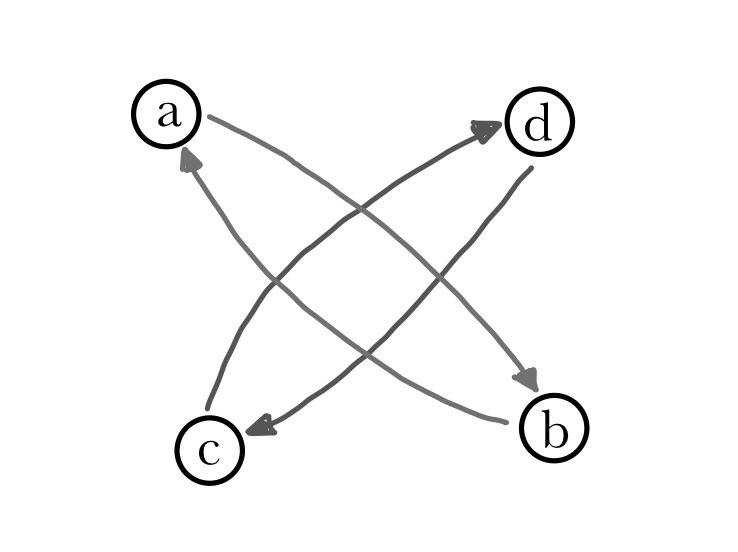
\includegraphics[scale=.20]{img/nocross.jpg}
\caption{(no-cross constraints explained) if there is a cable connecting $a$ and $b$, a cable starting (or ending) in $c$ cannot be laid if this one passes between $a$ and $b$.}
\label{img:noCross}
\end{figure}

However, following \cite{FISCHETTI2018917}, the number of constraints can be reduced to be $O(n^3)$ considering triples of points.
Let $(a,b,c)$ be such a triple, then, if a cable has been set between $a$ and $b$, it is necessary to avoid introducing cables starting (or ending) in $c$ and crossing the edge $\{a,b\}$.

A more exhaustive description of these constraints and a formal proof of their validity for the model can be found here \cite{FISCHETTI2018917}. Adhering to this description, let $\mathcal{C} \subset A \times A$ be \emph{the set of couples of edges that intersect each other}. We can define the clique arc subset $\mathcal{Q}$ as
\begin{gather}
\label{eqn:QSet}
\mathcal{Q}(a,b,k) = \left\{(a,b),(b,a)\right\} \cup \left\{(k,h) \in A : (\{a,b\},\{k,h\}) \in \mathcal{C}\right\}
\end{gather}

Finally, we introduce the no-cross constraints:
\begin{gather}
\label{eqn:noCrossConstraints}
\sum_{(i,j)\in \mathcal{Q}(a,b,k)} y_{i,j} \le 1 \quad a,b,k \in V,\,|\{a,b,k\}|=3 
\end{gather}

A note about performance. Although with the method we described the amount of constraints is reduced to $O(n^3)$, the number of operations required to compute them is still $O(n^4)$.

Clearly, this is irrelevant if the constraints are generated once. However, some applications we developed need to generate or check no-cross constraints numerous times. In this case, we think the best solution is to implement a \emph{look-up table} that, for every couple of edges, returns if they intersect or not.\\

Let consider the instance with $n = 100$ turbines (worst case in this report), in order to save the information for the table it would be necessary to maintain $100^4\,bytes$ (approximately $95\,Mbytes$).
By wasting one byte to store a boolean value, we do not achieve satisfying management of space. By means of more efficient data structures, we reduced that quantity to approximately $3\,Mbytes$.

Although this could seem quite a large value, it is sufficient to fit the look-up table in the cache of most commercial processors.


\subsection{Relaxed Model}
\label{sec:relaxedModel}

We introduce now a relaxed variant of the model previously described: this allows \texttt{CPLEX} to find an initial incorrect solution, namely a solution violating the model (\ref{eqn:MILPModelStart}) - (\ref{eqn:noCrossConstraints}), yet in a short amount of time.
Nevertheless, the cost of a relaxed solution will be such that \texttt{CPLEX} will always look for a solution restricted by constraints of the original model.

In order to obtain such variant, we include two kinds of relaxed constraints:
\begin{itemize}
\item \emph{substation in-degree relaxation}, that allows the substation to receive more input cables, violating the limit imposed by $C$;
\item \emph{cable flows relaxation}, with this artifice it is possible to admit disconnected solutionts.
\end{itemize}

For the first one, we change equation (\ref{eqn:substationInDegConstraint}) introducing the slack variable $s$
\begin{gather}
\label{eqn:substationInDegConstraintRelax}
\sum_{i=1}^n y_{i,h} - s\le C, \quad \forall\,h\in V : P_h = -1\\
s \ge 0, \; s \; integer.
\end{gather}

For the second relaxation, we modify equations (\ref{eqn:flowsContraints}) as:
\begin{gather}
\label{eqn:flowsConstraintsRelaxed}
\sum_{l=1}^n \left(f_{h,l} - f_{l,h}\right) + l_h= P_h, \quad \forall\,h \in V : P_h \ge 0\\
\label{eqn:extendedMILPModelEnd}
0 \le l_h \le k_{MAX}, \quad \forall\,h \in V : P_h \ge 0
\end{gather}
where $k_{MAX}$ is the maximum cable capacity.

The coefficients of variables $s$ and $l_h$ in the objective function are fixed to $M \gg 0$, a sufficiently large value.


\newpage


\section{Implementing and Solving the Model with CPLEX}
\label{sec:implementingAndSolvingWithCPLEX}


In order to solve the problem introduced earlier, we used different types of algorithms.
As can be seen from section \ref{sec:noCrossConstraints}, the main obstacle for a solver is represented by the high number of constraints used to deny that the cables intersect each other.
Even for a state-of-the-art LP and MILP solver as \texttt{CPLEX}, it could be surprisingly difficult to obtain an acceptable solution in a reasonable amount of time when the number of turbines is greater than 70 or 80.

Consequently, to circumvent this complication, we developed and analyzed different approaches.
Some of these methods require \texttt{CPLEX}, however, we also provided heuristic algorithms.\\

The algorithms can be divided into three classes, each representing a different paradigm:
\begin{itemize}
\item \emph{exact};
\item \emph{matheuristic};
\item \emph{heuristic}.
\end{itemize}

Solvers handling exclusively \texttt{CPLEX} features belong to the first class. These ones try to solve the problem optimally, but they could employ a huge amount of time to prove that a solution is the optimal one.

Instead, algorithms using \texttt{CPLEX} in order to obtain intermediate solutions, reside to the matheuristic class. With this approach, optimality is not guaranteed still it is much simpler to find a valid solution.

At last, we dedicate the next chapter to explain and analyze our heuristic algorithms.

\subsection{Extact Solvers}

\texttt{IBM ILOG CPLEX} \cite{IBMILOGCPLEX_manual} is an extremely powerful optimization software providing a large number of features and configurations.
\texttt{CPLEX} can be used as an interactive solver, indeed thanks to its command line interface, the user can furnish a file containing a model, set parameters and ask \texttt{CPLEX} to find a solution.
However, \texttt{CPLEX} provides lower level accesses interfacing with most widespread programming languages, such as C, C++, Java, C\# and Python.

In the present work, we exclusively discuss the approach with the \emph{CPLEX Callable Library} (CCL) that is the interface provided for the C and C++ programming languages.\\

\subsubsection{Basic Guide to CPLEX}

As can be guessed from the title, this does not want to be an exhaustive guide to all the secrets concerning \texttt{CPLEX} but rather a tutorial that helps a novice user in modelling problems with this software.
For a more detailed discussion, we recommend consulting the \emph{CPLEX User's Manual} \cite{IBMILOGCPLEX_manual} and the product website \cite{IBMILOGCPLEX_web}.\\

First of all, it is necessary to define an environment in which to operate and the \texttt{CPXopenCPLEX} function fulfils this task.
The type \texttt{CPXENVptr} we obtain represents an environment that keeps information about the parameters we set.

The next step requires the initialization of a new problem with \texttt{CPXcreateprob} that returns a \texttt{CPXLPptr} pointer: this represents the key to access all data regarding our problem throughout the code we develop.
These two components we just created (or at least the \texttt{CPLEX} environment) are required by every \texttt{CPLEX} function.

Next, we need to generate the MILP model or, in other words, we require a procedure to translate the abstractions of the mathematical model into constraints and variables that \texttt{CPLEX} is able to deal with.
Conventionally, in linear programming a variable is represented by a column of the matrix while a constraint is represented by a row.
Adopting this convention, the CCL provides the \texttt{CPXnewcols} function to add one or more columns to the model.

This function allows the user to set:
\begin{itemize}
\item the \textbf{number of columns} the user wants to add;
\item the \textbf{objective function coefficients};
\item the \textbf{lower bounds};
\item the \textbf{upper bounds};
\item the \textbf{types} of the variables (\emph{binary}, \emph{continuous}, \emph{integer}, \emph{semi-continuous} or \emph{semi-integer});
\item the \textbf{names}, this makes it easier to distinguish a variable.
\end{itemize}

According to model (\ref{eqn:MILPModelStart}) - (\ref{eqn:extendedMILPModelEnd}), we divide variables into five classes, assigning them different names:
\begin{itemize}
\item $f(i,j)$, continuous non-negative variables representing the flow running in the edge $(i,j) \in A$;
\item $x(i,j,k)$, binary variables representing the choice of the cable in the edge $(i,j) \in A$, $\forall\,k$, $1\le k \le K$;
\item $y(i,j)$, binary variables representing if the edge $(i,j) \in A$ must be built or not;
\item $s$, integer non-negative variable, it is used to relax the substation input degree constraint;
\item $l(h)$, continuous non-negative variables $\forall\,h\in V$, these are employed to relax the flow constraints.
\end{itemize}
The coefficients of the $f$ and $y$ variables are clearly $0$, instead, the coefficients of the $x(i,j,k)$ variables are given by the length of cable $(i,j)$  multiplied by the unitary cost of the $k$-th cable.
As said in their dedicated subsection, the $s$ and $l$ variables should not be chosen by the solver, thus their coefficient must be a very high value and we retain $10^{12}$ could be large enough for our purposes.

The total number of variables is $n^2(K + 2) + n + 1$ and this quantity is definitely dominated by the number of the $x$ variables.\\

Within \texttt{CPLEX} a constraint is represented by a row, then the \texttt{CPXnewrows} function permits the user to add one or more constraints. It is possible to set the following parameters:
\begin{itemize}
\item the \textbf{number of rows} the user wants to add;
\item the \textbf{right-hand-sides} of the rows;
\item the \textbf{senses} (\emph{lower or equal}, \emph{equal}, \emph{greater or equal}, \emph{ranged});
\item the \textbf{range values};
\item the \textbf{names}.
\end{itemize}

When a new row is appended to the model, its coefficients are fixed to zero by default.
The \texttt{CPXchgcoef} routine is required to change one coefficient of the matrix providing the \textbf{row's index}, the \textbf{column's index}, and the coefficient's \textbf{new value}.
Other useful functions in this phase are \texttt{CPXgetnumcols} and \texttt{CPXgetnumrows} that respectively provide the current number of columns and the current number of rows constituting the matrix.

Once understanding the theoretical model, the implementation of its constraints through \texttt{CPLEX} should be quite straightforward, therefore we do not spend further words in technical details.\\

We consider the default model for our purposes the one composed of the (\ref{eqn:MILPModelStart}) - (\ref{eqn:MILPModelEnd}) equations while the (\ref{eqn:substationInDegConstraintRelax}) - (\ref{eqn:extendedMILPModelEnd}) equations can be added or removed by fixing their two related parameters in our software.
No-cross constraints (\ref{eqn:noCrossConstraints}) are not included in the default model because we developed several procedures to append them and each procedure possesses pro and cons we desire to analyse.\\

Before trying to launch the solver, the user can choose to set several among the large number of parameters \texttt{CPLEX} makes available.
This can be done by using \texttt{CPXsetintparam}, \texttt{CPXsetlongparam} or \texttt{CPXsetdblparam} functions depending on whether the parameter we want to access is respectively an integer, a long integer or a double type.

For example, one of the most common parameters a user would like to fix is certainly the computation time limit. The command
\begin{lstlisting}[style=C]
	CPXsetdblparam(env, CPX_PARAM_TILIM, 60.0);
\end{lstlisting}
sets parameter \texttt{CPX\_PARAM\_TILIM} (that is a double type) to $60$ seconds in the \texttt{env} environment.

The calculation starts when the \texttt{CPXmipopt} function is called.
At this point, other choices are available, for example, if a model does not contain binary or integer variables, the \texttt{CPXlpopt} routine must be used.

At the expiry of the time limit chosen by the user, \texttt{CPLEX} may not have found a solution, in this case, the \texttt{CPXgetx} function throws an error.
Otherwise, it allows getting a vector containing the values of each variable in the best solution found until that time.
Other useful information at the end of the computation can be found with \texttt{CPXgetbestobjval}, that returns the value of the best known bound on the optimal solution value, and \texttt{CPXgetobjval}, that provides the solution objective value.

The user can also save the model to an \emph{LP file}\cite{LPfile} in every moment after generating it with the \texttt{CPXwriteprob} routine.

Finally, when the model is no longer needed, the user must free it with \texttt{CPXfreeprob}.
Afterwards, it is necessary to call the \texttt{CPXcloseCPLEX} function to close the \texttt{CPLEX} environment.

\subsection{Adding No-cross Constraints}

\subsubsection{Lazy Constraints}

After importing the mathematical model in \texttt{CPLEX}, we needed a procedure to generate constraints (\ref{eqn:noCrossConstraints}).
Consequently, we implemented the \emph{generateNoCrossConstraints} routine as described in Algorithm \ref{alg:generateNoCrossConstraints}: as can be seen, the addConstraint command is a general one and it does not furnish implementation details.
Clearly, this command can be realized with the \texttt{CPXaddnewrows} function and we tried this method for comparison purposes.

Nevertheless, \texttt{CPLEX} provides also a different technique to append a new constraint to the model.
The \texttt{CPXaddlazyconstraints} function works in a similar way as \texttt{CPXaddnewrows}, yet it should be used to add a large set of constraints that must be satisfied in the final solution but are unlikely to be really violated.
In fact, the function creates and appends a constraint to the model only when the solver discovers that this can be actually violated.


\begin{algorithm}[h]
\caption{\emph{generateNoCrossConstraints} procedure.}
\label{alg:generateNoCrossConstraints}
\SetKwData{Left}{left}\SetKwData{This}{this}\SetKwData{Up}{up}
\SetKwFunction{Union}{Union}\SetKwFunction{FindCompress}{FindCompress}
\SetKwInOut{Input}{input}\SetKwInOut{Output}{output}
\Input{$turbs$, a vector of cartesian points; $lpModel$, a linear programming model.}
\Output{$lpModel$ extended with no-cross constraints.}
\BlankLine
%%
\For{$i \gets 1$ \KwTo n}
{
	\For{$j \gets 1$ \KwTo n}
	{
		\For{$k \gets 1$ \KwTo n}
		{
			$S \gets \emptyset$\\
			\For{$l \gets 1$ \KwTo n}
			{
				\If{$isCrossing(turbs[i], turbs[j], turbs[k], turbs[l])$}
				{
					$S \gets S \cup \{l\}$\\
				}
			}
			
			\If{$\left|S\right| > 0$}
			{
				$lpModel.addConstraint\left(y_{i,j} + \sum_{l \in S}y_{k,l} \le 1\right)$\\
			}
		}
	}
}
%%
\end{algorithm}


\begin{algorithm}[h]
\caption{\emph{isCrossing} procedure.}
\label{alg:isCrossing}
\SetKwData{Left}{left}\SetKwData{This}{this}\SetKwData{Up}{up}
\SetKwFunction{Union}{Union}\SetKwFunction{FindCompress}{FindCompress}
\SetKwInOut{Input}{input}\SetKwInOut{Output}{output}
\Input{$p1$, $p2$, $p3$, $p4$ cartesian points with $x$ and $y$ attributes; $\epsilon > 0$, tolerance parameter.}
\Output{$1$ if segments $(p1,p2)$ and $(p3,p4)$ cross each other, $0$ otherwise.}
\BlankLine
%%
$a \gets p1.x - p2.x$\\
$b \gets p4.x - p3.x$\\
$c \gets p1.y - p2.y$\\
$d \gets p4.y - p3.y$\\
$e \gets p4.x - p2.x$\\
$f \gets p4.y - p2.y$\\
$det \gets a \cdot d - b \cdot c$\\

\If{ $\left|det\right| < \epsilon$ }
{
	% no crossing
	\textbf{return} 0\\
}	
\Else
{
	$\lambda \gets (d \cdot e - b \cdot f)\,/\,det$\\
	$\mu \gets (a \cdot f - c \cdot e)\,/\, det$\\
	
	\If{ $(0 < \lambda < 1) \wedge (0 < \mu < 1)$ }
	{
		% crossing
		\textbf{return} 1\\
	}
	\textbf{return} 0\\
}
%%
\end{algorithm}


\subsubsection{Callbacks}

A different technique to discover violated constraints and joining them to the model \emph{on-the-fly} involves the \emph{callbacks}.
In general, a callback is a user-defined function $X$ that is passed as a parameter to another function $Y$.
For example, $Y$ could be a general purpose function that utilizes $X$ in order to accomplish specific operations on user-defined data whose details were not available during $Y$'s implementation.\\

By means of this technique, \texttt{CPLEX} allows the user to define functions for his specific purposes and these functions can be called during the optimization process.
\texttt{CPLEX} provides several kinds of callbacks, nevertheless here we only show how to deal with the ones allowing to add the \emph{lazy constraints}.
In the following are reported the steps that should be followed when using callbacks in \texttt{CPLEX}.
\begin{itemize}
\item \textbf{Installing the callback}: this task can be accomplished by using the \texttt{CPXsetlazyconstraintcallbackfunc} function that receives as arguments the callback the user has defined and the data needed for its computation (in our specific case, we send the positions of the turbines).
\item \textbf{Obtaining information}: plenty of useful information can be obtained during the computation by calling the \texttt{CPXgetcallbackinfo} routine.
For example, by passing the \texttt{CPX\_CALLBACK\_INFO\_MY\_THREAD\_NUM} parameter, the user-defined function can identify the thread in which it is running.
\item \textbf{Performing specific subroutines:} inside a callback, the user is able to specify any sort of operation she requires for her purposes, remembering that the making use of data provided as a parameter to the callback, must be managed in a thread-safe environment.
\item \textbf{Adding the cuts}: after generating a useful cut (o more than one), the user can append it to the model by invoking the \texttt{CPXcutcallbackadd} function. The successful production of at least one cut must be notified to \texttt{CPLEX} with the following line of code
\begin{lstlisting}[style=C]
	*useraction_p = CPX_CALLBACK_SET;
\end{lstlisting}
where \texttt{useraction\_p} is the last parameter in the definition of a callback.
\end{itemize}


\subsubsection{Loop Method}

Being a large amount of no-cross constraints our main complication, we can design a simple procedure that appends to the model only the ones really required by the instance.
A precise description of our implementation for the so called \emph{Loop Method} is given by Algorithm \ref{alg:LoopMethod}.

The procedure invokes \texttt{CPLEX} with an extremely short time limit ($30$ seconds is generally enough for our testbed) in order to solve the model (initially without no-cross constraints). 
Subsequently, it checks the solution obtained in the previous step, appending the violated constraints to the model.

These two main steps are iterated until the time limit is reached.


\begin{algorithm}[H]
\caption{The \emph{Loop Method} pseudocode.}
\label{alg:LoopMethod}
\BlankLine
initialize \emph{model} without no-cross constraints\\
\While{\emph{time limit not reached}}
{
	$solution \gets$ solve \emph{model} within a time limit $T$ and get a solution\\
	\If{\emph{$solution$ is an integer feasible solution}}
	{
		\For{\emph{\textbf{each} $(i,j,k) \in V\times V\times V$}}
		{
			$S \gets \emptyset$\\
			\For{$l \gets 1$ \KwTo n}
			{
				\If{\emph{$y_{i,j} \in solution$ \textbf{and} $y_{k,l} \in solution$ \textbf{and}  $isCrossing(turbs[i], turbs[j], turbs[k], turbs[l])$}}
				{
					$S \gets S \cup \{l\}$\\
				}
			}
			
			\If{$\left|S\right| > 0$}
			{
				$model.addConstraint\left(y_{i,j} + \sum_{l \in S}y_{k,l} \le 1\right)$\\
			}
		}
	}
}
\end{algorithm}

\newpage

% DA RIVEDERE
\section{Heuristic and Matheuristic Solvers}
\label{sec:HeuristicSolvers}

In this chapter, we cover several ideas to solve our original problem nevertheless, these do not guarantee to find an optimal solution.
Techniques that make use of \emph{rules of thumb} (specifically designed for a problem), fall under the name of \emph{heuristics}.

\subsection{Hard-fixing}

A relatively new approach to optimization is provided by \emph{matheuristic algorithms}.
Matheuristic is a collection of techniques that combine the power of mathematical solvers with the intuition of heuristic and \emph{metaheuristic} algorithms (see \cite{10.1007/978-3-642-04918-7_13}).
We investigated one method belonging to this family, named \emph{Hard-fixing}.\\

After generating the model (\ref{eqn:MILPModelStart}) - (\ref{eqn:extendedMILPModelEnd}), the \emph{Hard-fixing} procedure calls \texttt{CPLEX} to gain a starting, even infeasible, solution and by means of the slack variables, this is achievable within a small interval of time.

Afterwards, the algorithm examines the $y$ variables and it randomly fixes an arbitrary percentage of such variables.
This action is performed by changing the bounds of chosen variables: for example, if a variable is set to $1$ in the solution found by \texttt{CPLEX}, we change its upper and lower bound to $1$ (this can be performed with the \texttt{CPXchgbds} function).
Subsequently, \texttt{CPLEX} is newly called to solve the model thus obtained.

These steps are repeatedly executed until a time limit expires or no improvements can be achieved.


\begin{algorithm}[H]
\caption{The \emph{Hard-fixing} pseudocode.}
\label{alg:HardFixing}
\BlankLine
initialize \emph{model}\\
\While{\emph{time limit not reached}}
{
	$solution \gets$ solve \emph{model} within a time limit $T$ and get a solution\\
	% hard-fix
	\For{$i \gets 1$ \KwTo $n$}
	{
		\For{$j \gets 1$ \KwTo $n$}
		{
			reset lower and upper bounds in \emph{model} as $0 \le y_{i,j} \le 1$\\
			\If{$rand() > FIXING\_PROB$}
			{
				\eIf{\emph{$y_{i,j} = 0$ in \emph{solution}}}
				{
					set $0 \le y_{i,j} \le 0$ in \emph{model}\\
				}{
					set $1 \le y_{i,j} \le 1$ in \emph{model}\\
				}
			}
		}
	}
}
\end{algorithm}

\subsection{Pure Heuristic Approaches}

Branch-and-bound technique and mixed integer linear programming are undoubtedly effective approaches, yet their time complexity is high and unacceptable in certain circumstances.
Moreover, the implementation of a practical MILP solver is usually a task beyond the possibilities of a computer engineer and software like \texttt{CPLEX} might be really expensive.

To overcome these problems one can use \emph{heuristic algorithms}, designed to solve a problem in a faster and more efficient fashion than traditional methods by sacrificing optimality for speed.

Heuristics are often used to solve NP-hard problems, for which there is not an efficient way to find a solution in a short time.

Heuristic algorithms can certainly produce suitable solutions, nevertheless, they can also be employed to provide good baselines to feed supplemented optimization algorithms.
\texttt{CPLEX} is a good example of the latter approach, indeed, it makes available to the user several heuristic routines that can be launched during the computation.
The most known and successful of these techniques is the \emph{Relaxation Induced Neighborhood Search} (RINS) \cite{Danna2005}, a method for exploring the neighbourhood of the current incumbent solution in order to find an improved one.\\

%Therefore, heuristics are most often employed when approximate solutions are sufficient and exact solutions are too computationally expensive.

Below, we describe some auxiliary functions, useful for understanding subsequent algorithms.
The pure heuristic routines we have implemented to solve this problem are a \emph{multi-start} (MS) approach and the \emph{Variable Neighborhood Search} (VNS).


\subsubsection{Clustering Tree Generation}

This function was created in order to avoid starting an optimization routine with a \emph{star graph}, namely a solution in which each turbine is directly connected to the substation.
The star graph solution is clearly incorrect because the number of cables entering the substation overcomes our parameter $C$.

Therefore, we opted to make use of a clustering method to obtain an initial solution that could be closer to our needs.

The algorithm we designed chooses $C$ randomly turbines that become the centres of the clusters in which the graph is subdivided. 
Then, it scans the remaining turbines and assigns each of them to its nearest centre. 
The centre of each cluster is directly connected to the substation.

The algorithm pseudocode is reported in Algorithm \ref{alg:clusteringTreeGeneration}.


\begin{algorithm}[H]
\caption{\emph{Clustering Tree Generation} pseudocode.}
\label{alg:clusteringTreeGeneration}
\SetKwData{Left}{left}\SetKwData{This}{this}\SetKwData{Up}{up}
\SetKwFunction{Union}{Union}\SetKwFunction{FindCompress}{FindCompress}
\SetKwInOut{Input}{input}\SetKwInOut{Output}{output}
\Input{\emph{turbs}, a vector containing the coordinates of the turbines; $C$, maximum number of cables the substation can accept.}
\Output{\emph{succ}, a structure containing for each turbine $i$ the \emph{successor} of $i$.}
\BlankLine
Initialize \emph{succ} and \emph{visited}, get the index of the substation from \emph{succ} and assign it to \emph{substationIndex}\\
\BlankLine
$succ[substationIndex] \gets substationIndex$\\
$visited[substationIndex] \gets 1$\\
\For{$i \gets 1$ \KwTo $n$}
{
	\For{$j \gets 1$ \KwTo $n$}
	{
		$M[i,j] \gets distance(turbs[i], turbs[j])$\\
	}
}
\BlankLine
$S \gets \emptyset$\\
\While{$\left|S\right| < C$}
{	
	$r \gets $ a random value in $\{1, \hdots, n\} / \left(S \cup \{substationIndex\}\right)$\\
	$visited[r] \gets 1$\\
	$succ[r] \gets substationIndex$\\
	$S \gets S \cup \{r\}$\\
}
\BlankLine
\For{$i \gets 1$ \KwTo n}
{
	\If{$\textbf{not } visited[i]$}
	{	
		$index \gets 0$\\
		$minDist \gets \infty$\\
		\For{$j \in S$}
		{	
			\If{$M[i,j] < minDist$}
			{
				$index \gets j$\\
				$minDist \gets M[i,j]$\\	
			}
		}
		$succ[i] \gets index$\\
		$visited[i] \gets 1$\\
	}
}
\textbf{return }$succ$\\
\end{algorithm}


% RIVEDERE
\subsubsection{The twoOpt and threeOpt Routines}

In our implementation, the \emph{twoOpt} routine is a local search algorithm that considers every path in the cables routing involving 2 connections and 3 turbines, choosing the solution that provides the best outcome (i.e., the minimum cost).

Actually, this is performed by means of an exhaustive search, examining all the $(i,j,k)$ triples in the $V^3$ search space and each of these triples matches a path $(y_{ij}, y_{jk})$.
In a similar way, the \emph{threeOpt} algorithm iterates over each tuple $(i,j,k,l) \in V^4$ and evaluates the solutions obtained replacing connections $y_{ij}$ and $y_{kl}$.

By changing the entries in the \emph{succ} structure, we are able to modify the connections in the cables routing: if we require turbine $i$ (and consequently, all the turbines in its subtree) to be joined to turbine $j$, we should perform 
\begin{center}
$succ[i] \gets j$.
\end{center}

This operation guarantees that the number of edges remains $n-1$ (the first entry in the \emph{succ} structure will be always ignored) but it allows the presence of loops.
In order to avoid them in the final layout, the evaluation phase assigns high penalties to solutions containing connections with cycles.

Both \emph{twoOpt} and \emph{threeOpt} return explicitly the value of the best solution found and implicitly the \emph{succ} structure matching such a solution.\\

The naming rule adopted by these routines was generated during the development phase.
In fact, according to this rule, \emph{oneOpt} is the most basic local search approach that can be accomplished, and it corresponds to modify the successor of each node, attempting to connect it to all the other turbines.

This process can be easily generalized by producing a \emph{$k$-Opt} routine that will generate $n^{k+1}$ different solutions.
Nevertheless, even if this number is not high, it should be remembered that each solution thus found must be evaluated.

\subsubsection{Solution Evaluation}

Clearly, the most onerous operation in the \emph{twoOpt} and \emph{threeOpt} routines is the evaluation of the new solutions found or, in other words, the evaluation of the \emph{succ} structure according to our mathematical model.
In order to achieve this task, we design an algorithm that accomplishes as fewer activities as possible.

The algorithm starts verifying if the solution is rightly connected and if the edges do not form any cycles.
Then it checks the flows in every edge, adding a penalty to the solution score for each flow that does not respect the constraint imposed by its edge.
Afterwards, the cables entering the substation are scanned while the last and harder step is the control of the no-cross constraints (\ref{eqn:noCrossConstraints}).

In order to avoid unnecessary operations, the value of the best solution found until that moment, is provided to the function computing the evaluation.
In this way, the evaluation can be arrested by several checkpoints located in strategic places, if the current score overcomes the best solution value.

\subsubsection{Multi-Start}

The first heuristic we tested on the cables routing problem was a \emph{multi-start} approach.
This is a quite straightforward method however, it was able to produce interesting results.

The procedure repeatedly tries to make small improvements until a local optimum point is reached.
Suddenly the best solution is preserved and a new starting basis is provided by the \emph{clusteringTreeGeneration} function with a different random seed, in order to produce a distinct basis.
The entire procedure terminates when a user-defined time limit is reached.
The algorithm pseudocode is reported in Algorithm \ref{alg:multistart}.

When the maximum number of cables entering the substation is not provided (i.e., this is infinite), a value proportional to the number of turbines can be chosen, however, for these cases, we set this parameter to 10.

Thanks to the chaotic structure of the problem, small changes in the starting cables routing can produce totally different outcomes and although an optimal solution is hardly reachable, providing a suitable initial base, usually enables to quickly generate feasible cables routings.\\

\begin{algorithm}[H]
\caption{\emph{Multi-start} approach pseudocode.}
\label{alg:multistart}
\SetKwData{Left}{left}\SetKwData{This}{this}\SetKwData{Up}{up}
\SetKwFunction{Union}{Union}\SetKwFunction{FindCompress}{FindCompress}
\SetKwInOut{Input}{input}\SetKwInOut{Output}{output}
\Input{\emph{turbs}, a vector containing the coordinates of the turbines; $C$, the maximum number of cables the substation can accept; \emph{succ}, an empty structure; the starting random \emph{seed}.}
\Output{\emph{minCost}, the value of the best solution found; (implicitly) \emph{succ}, a structure containing the best solution found.}

\BlankLine
\BlankLine
initialize structure \emph{bestSucc}\\
$minCost \gets \infty$\\
$iteration \gets 0$\\
\While{\emph{time limit not reached}}
{
	$seed \gets seed + iteration$\\
	set the system random seed to \emph{seed}\\
	$succ \gets clusteringTreeGeneration(turbs, C)$\\
	$improvement \gets 1$\\
	\While{\emph{improvement}}
	{
		$cost \gets twoOpt(succ, minCost)$\\
		$improvement \gets 0$\\
		\If{cost < minCost}
		{
			copy \emph{succ} to \emph{bestSucc}\\
			$improvement \gets 1$\\
			$minCost \gets cost$\\
		}
	}
}
copy \emph{bestSucc} to \emph{succ}\\
\textbf{return }$minCost$\\

\BlankLine
\BlankLine

\end{algorithm}

%\subsubsection{Simulated Annealing}
%
%The strategy of the SA algorithm aims at solving a usual problem in optimization, namely, avoiding that an optimization routine halts at a local optimum point.
%
%The concept of the annealing derived from the metallurgical industry where this process is used to eliminate the reticular defects of the crystals by means of a heating followed by slow cooling.\\
%
%We implemented this strategy in our optimization problem with the following passages (the related pseudocode is reported in Algorithm \ref{alg:simulatedAnnealing}).
%\begin{enumerate}
%\item An initial temperature equal to $T$ is set ($1$ is a usual choice for this parameter) and the subsequent steps are iterated:
%\begin{enumerate}
%\item a perturbation is introduced in the \emph{succ} structure (i.e., 2 random indices are set to as many random values);
%\item a slightly modified version of the \emph{twoOpt} routine is called in order to find a solution which cost is lower than $minCost\cdot(1+T)$ (we remember that this function returns explicitly the cost of the solution found and implicitly the \emph{succ} structure matching such solution);
%\item the algorithm discards the previously found solution (having cost \emph{minCost}) accepting the new one (associated with \emph{cost}) if the value of a uniform random variable distributed between 0 and 1 is greater than
%\begin{gather}
%\exp{\left\{\frac{minCost-cost}{T}\right\}}.
%\end{gather}
%\end{enumerate}
%\item The temperature is decreased (\emph{cooling phase}) in order to keep better solutions with higher probability and this continues until reaching the minimum temperature.
%\end{enumerate}
%
%
%\begin{algorithm}[H]
%\caption{\emph{Simulated Annealing} pseudocode.}
%\label{alg:simulatedAnnealing}
%\SetKwData{Left}{left}\SetKwData{This}{this}\SetKwData{Up}{up}
%\SetKwFunction{Union}{Union}\SetKwFunction{FindCompress}{FindCompress}
%\SetKwInOut{Input}{input}\SetKwInOut{Output}{output}
%\Input{\emph{succ}, a structure containing for each turbine $i$ the \emph{successor} of $i$; numerical parameters $numIterations$, $T$, $T_{min}$ and $\alpha$.}
%\Output{\emph{minCost}, the value of the best solution found}
%
%\BlankLine
%\BlankLine
%%$T \gets 1$\\
%%$T_{min} \gets 0.0001$\\
%$minCost \gets \infty$\\
%
%\While{$T > T_{min}$}
%{
%	\For{$i \gets 1$ \KwTo numIterations}
%	{
%		insert a random perturbation in \emph{succ}\\
%		$cost \gets twoOpt(succ, minCost\cdot(1+T))$\\
%		$keep \gets $ choose to take or not the solution with probability proportional to $\exp{\left\{\frac{minCost - cost}{T}\right\}}$\\
%		\If{keep}
%		{
%			$minCost \gets cost$\\
%		}
%	}
%	\textbf{comment: }\emph{cooling phase}\\
%	$T \gets \alpha \cdot T$\\
%}
%\textbf{return }$minCost$\\
%
%\BlankLine
%\BlankLine
%
%\end{algorithm}


\subsubsection{Variable Neighborhood Search}

This heuristic algorithm bases its strategy on the local search: it first discovers a local optimum point and then upsets this solution in order to escape from such a point and try to reach the global optimum one.

In the variant of the procedure we designed, we start from an initial solution given by the \emph{Dijkstra algorithm} (a description of this algorithm can be found in \cite{fischetti1995lezioni}), such a solution is then provided to the VNS routine.
The VNS changes one connection at a time, saving it whenever improvements are encountered.
When no further advancements can be found, the \emph{threeOpt} routine is launched, trying to escape from the local optimum point.

The solution obtained with the Dijkstra algorithm can be randomized to obtain different starting basis and repeat the entire procedure in order to achieve different results.
The way we modified the Dijkstra algorithm is extremely simple. This algorithm bases its choice on the costs of the edges hence, we change the cost of each edge proportionally to its length, by adding a random perturbation to increment or decrement it.\\


\begin{algorithm}[H]
\caption{\emph{Variable Neighborhood Search} pseudocode.}
\label{alg:VariableNeighborhoodSearch}
\SetKwData{Left}{left}\SetKwData{This}{this}\SetKwData{Up}{up}
\SetKwFunction{Union}{Union}\SetKwFunction{FindCompress}{FindCompress}
\SetKwInOut{Input}{input}\SetKwInOut{Output}{output}
\Input{\emph{succ}, a structure containing for each turbine $i$ the \emph{successor} of $i$.}
\Output{\emph{minCost}, the value of the best solution found; (implicitly) \emph{succ}, a structure containing the best solution found.}

\BlankLine
\BlankLine

$minCost \gets \infty$\\
\While{1}
{
	$currentMinCost \gets minCost$\\

	\For{$i \gets 1$ \KwTo n}
	{
		\For{$j \gets 1$ \KwTo n}
		{
			$tmp \gets succ[i]$\\
			$succ[i] \gets j$\\
			$cost \gets evaluate(succ)$\\
			\eIf{cost < currentMinCost}
			{
				$currentMinCost \gets cost$\\
			}{
				$succ[i] \gets tmp$\\
			}
		}
	}
	
	\eIf{currentMinCost < minCost}
	{
		\textbf{comment: }\emph{local optimum not reached, update cost and repeat the previous routine}\\
		$minCost \gets currentMinCost$\\
	}{
		\textbf{comment: }\emph{local optimum reached}\\ 
		$cost \gets threeOpt(succ)$\\
		
		\If{$minCost \le cost$}
		{
			\textbf{return }$minCost$\\
		}
	}
}

\BlankLine
\BlankLine

\end{algorithm}



\newpage

% CORRETTO TUTTO
\section{Results}
\label{sec:results}

The real world cases we considered for this study were obtained from the wind farms listed in Table \ref{tab:windfarms}.
Assigning them different sets of cables, we produced the testbed for our experiments with 24 instances as reported in Table \ref{tab:testbed}.

In addition to the original cables (\emph{cb01} to \emph{cb05}) denominated CAPEX (CAPital EXpenditure), since these are only considered as an immediate expense, the authors of the article \cite{FISCHETTI2018917} developed other sets of cables estimating future costs.
In this way, for each of the original sets of cable (now reporting the \emph{capex} suffix), a new one was obtained in order to compare the different solutions.\\

We carried out our experiments on a personal computer equipped with an Intel i3 CPU 530, 2.93 GHz x4, 7.7 GB RAM memory and the \texttt{IBM ILOG CPLEX 12.8} software.\\

\begin{table}[H]
\begin{center}
\begin{tabular}{rlrrl}
\hline
Name & Site & n. of turbines & C & Allowed cables\\
\hline
wf01 & Horns Rev 1   & 80  & $10$     & cb01-cb02-cb05\\
wf02 & Kentish Flats & 30  & $\infty$ & cb01-cb02-cb03-cb04-cb05\\
wf03 & Ormonde       & 30  & $4$      & cb03-cb04\\
wf04 & DanTysk       & 80  & $10$     & cb01-cb03-cb04-cb05\\
wf05 & Thanet        & 100 & $10$     & cb04-cb05
\end{tabular}
\end{center}
\caption{The real wind farms we considered (from \cite{FISCHETTI2018917}).}
\label{tab:windfarms}
\end{table}

The results were obtained by running each instance with a 3600 seconds time limit.
Therefore, these have been compared with the results produced through other similar techniques or different configurations.

Consequently, we do not record the values of infeasible solutions and we report beside each result the error as compared to the best lower bound known (the optimal solution found for the same instance by Fischetti and Pisinger in \cite{FISCHETTI2018917}).
This error is calculated as
\begin{gather*}
\left(1-\frac{LB}{val}\right) \cdot 100.
\end{gather*}

In Table \ref{tab:LazyNewrowsNoSlack}, we reported the data obtained generating all the constraints (\ref{eqn:noCrossConstraints}) by means of the \emph{lazy constraints} and the \emph{new rows}. 
As it can be seen, the model (\ref{eqn:MILPModelStart}) - (\ref{eqn:noCrossConstraints}) without slack variables can be used to solve the smaller cases, however the problem becomes unmanageable in cases with 80 or 100 turbines (the software was sometimes stopped by the operating system before reaching the time limit).

The main difference in using the \emph{lazy constraints} instead of the \emph{new rows} is that the former results to be much faster than the latter.
This fact can be observed in instances 9, 12 and 14.

Through these examples, we can also notice that \texttt{CPLEX} stops the computation after finding the optimal solution according to the model and the data we provided. Nevertheless, the gap between the solution we found and the solution in \cite{FISCHETTI2018917} is not exactly zero due to internal \texttt{CPLEX}'s tolerances.\\

%testbed
\begin{table}[H]
\begin{adjustwidth}{-.5in}{-.5in}
\begin{center}
\begin{tabular}{ll}
\begin{tabular}{r|cl}
\hline
Inst. & Wind farm & Cable set\\
\hline
 1 & \multirow{6}{*}{wf01} & wf01\_cb01\_capex\\
 2 &                       & wf01\_cb01\\
 3 &                       & wf01\_cb02\_capex\\
 4 &                       & wf01\_cb02\\
 5 &                       & wf01\_cb05\_capex\\
 6 &                       & wf01\_cb05\\
\hline
 7 & \multirow{6}{*}{wf02} & wf02\_cb01\_capex\\
 8 &                       & wf02\_cb01\\
 9 &                       & wf02\_cb02\_capex\\
10 &                       & wf02\_cb02\\
11 &                       & wf02\_cb03\\
13 &                       & wf02\_cb04\\
\end{tabular}

&

\begin{tabular}{r|cl}
\hline
Inst. & Wind farm & Cable set\\
\hline
14 & \multirow{2}{*}{wf02} & wf02\_cb05\_capex\\
15 &                       & wf02\_cb05\\
\hline
16 & \multirow{4}{*}{wf03} & wf03\_cb03\_capex\\
17 &                       & wf03\_cb03\\
18 &                       & wf03\_cb04\_capex\\
19 &                       & wf03\_cb04\\
\hline
20 & \multirow{2}{*}{wf04} & wf04\_cb01\_capex\\
21 &                       & wf04\_cb01\\
\hline
26 & \multirow{4}{*}{wf05} & wf05\_cb04\_capex\\
27 &                       & wf05\_cb04\\
28 &                       & wf05\_cb05\_capex\\
29 &                       & wf05\_cb05
\end{tabular}
\end{tabular}
\end{center}
\end{adjustwidth}
\caption{The testbed considered in this report.}
\label{tab:testbed}
\end{table}


% lazy constraints and new rows no slack
\begin{table}[H]
\begin{adjustwidth}{-2.4in}{-2.4in}
\begin{center}
\begin{tabular}{r|rrr|rrr}
\hline
Inst. & \multicolumn{2}{l}{Lazy constraints} & & \multicolumn{2}{l}{New rows} & \\ 
& Time & bestsol & \% err. &  Time & bestsol & \% err. \\ 
\hline
1  & 3600.75 & -           & -    & 3602.66 & -           & -    \\
2  & 3602.65 & -           & -    & 3600.00 & -           & -    \\
3  & 3600.77 & -           & -    & 3604.17 & -           & -    \\
4  & 3602.80 & -           & -    & 3600.00 & -           & -    \\
5  & 3600.65 & -           & -    & 3600.00 & -           & -    \\
6  & 3603.39 & -           & -    & 3600.00 & -           & -    \\
7  & 3600.04 & 8555171.40  & 0.00 & 3602.21 & 8555171.40  & 0.00 \\
8  & 3600.57 & 8806839.00  & 0.00 & 3600.08 & 8806839.00  & 0.00 \\
9  & 4.30    & 11159487.98 & 9.88 & 1903.35 & 11159487.98 & 9.88 \\
10 & 3600.04 & 10303320.45 & 0.00 & 3600.11 & 10303320.45 & 0.00 \\
12 & 8.07    & 9009167.55  & 4.49 & 3409.50 & 9009167.55  & 4.49 \\
13 & 706.51  & 8933494.43  & 0.00 & 1298.37 & 8933494.43  & 0.00 \\
14 & 39.05   & 10377051.63 & 1.96 & 3091.89 & 10377051.63 & 1.96 \\
15 & 3600.06 & 10348430.55 & 0.00 & 3600.11 & 10348430.55 & 0.00 \\
16 & 3600.06 & 8054844.90  & 0.00 & 3600.11 & 8054844.90  & 0.00 \\
17 & 3600.08 & 8560008.61  & 0.00 & 3600.09 & 8560008.61  & 0.00 \\
18 & 3600.07 & 8357195.91  & 0.00 & 3600.10 & 8357195.91  & 0.00 \\
19 & 3600.07 & 9178499.87  & 0.00 & 3600.13 & 9178499.87  & 0.00 \\
20 & 3600.72 & -           & -    & 3603.23 & -           & -    \\
21 & 3605.56 & -           & -    & 3600.00 & -           & -    \\
26 & 10.95   & -           & -    & 365.78  & -           & -    \\
27 & 3604.24 & -           & -    & 3612.16 & -           & -    \\
28 & 11.15   & -           & -    & 290.77  & -           & -    \\
29 & 3607.85 & -           & -    & 3600.00 & -           & -   
\end{tabular}
\end{center}
\end{adjustwidth}
\caption{Results comparison for \emph{lazy constraints} and \emph{new rows}, not involving callbacks.}
\label{tab:LazyNewrowsNoSlack}
\end{table}


Differently from what can seen above, the relaxation of the model implies a general slowdown in the computation (Table \ref{tab:LazyNewrowsWithSlack}).

Nevertheless, acceptable solutions can be calculated within the time limit for the \emph{Horns Rev 1} wind farm (which counts 80 turbines) and for the Thanet wind farm (instance 27, with 100 turbines).\\


% lazy constraints and new rows with slack
\begin{table}[H]
\begin{adjustwidth}{-2.4in}{-2.4in}
\begin{center}
\begin{tabular}{r|rrr|rrr}
\hline
Inst. & \multicolumn{2}{l}{Lazy constraints} & & \multicolumn{2}{l}{New rows} & \\ 
& Time & bestsol & \% err. &  Time & bestsol & \% err. \\ 
\hline
1  & 3601.45 & 19624392.92 & 0.96 & 3603.21 & 19549735.53 & 0.58 \\
2  & 3601.29 & 21509919.98 & 0.50 & 3603.43 & 21486462.37 & 0.39 \\
3  & 3600.99 & 23120440.28 & 2.20 & 3603.60 & 22616959.38 & 0.02 \\
4  & 3601.45 & 25316975.42 & 3.44 & 3603.74 & 24931979.39 & 1.95 \\
5  & 3600.97 & 24505448.34 & 4.17 & 3602.86 & 23631255.96 & 0.63 \\
6  & 3601.59 & 24877152.27 & 0.44 & 3603.48 & 25349299.98 & 2.29 \\
7  & 3600.06 & 8555171.40  & 0.00 & 3600.10 & 8555171.40  & 0.00 \\
8  & 3600.08 & 8806839.00  & 0.00 & 3600.10 & 8806839.00  & 0.00 \\
9  & 2052.98 & 11159487.98 & 9.88 & 3600.09 & 11159487.98 & 9.88 \\
10 & 3600.07 & 10303320.45 & 0.00 & 3600.09 & 10303320.45 & 0.00 \\
12 & 3600.06 & 9009167.55  & 4.49 & 3600.11 & 9009167.55  & 4.49 \\
13 & 3600.08 & 8933494.43  & 0.00 & 1633.34 & 8933494.43  & 0.00 \\
14 & 3600.05 & 10377051.63 & 1.96 & 3600.12 & 10377051.63 & 1.96 \\
15 & 3600.09 & 10348430.55 & 0.00 & 3600.14 & 10348430.55 & 0.00 \\
16 & 3600.06 & 8054844.90  & 0.00 & 3600.09 & 8054844.90  & 0.00 \\
17 & 3600.08 & 8560008.61  & 0.00 & 3600.14 & 8560008.61  & 0.00 \\
18 & 3600.05 & 8357195.91  & 0.00 & 3600.10 & 8357195.91  & 0.00 \\
19 & 3600.09 & 9178499.87  & 0.00 & 3600.11 & 9178499.87  & 0.00 \\
20 & 3601.10 & 38977593.84 & 0.00 & 3603.72 & 39779972.34 & 2.02 \\
21 & 3601.02 & -           & -    & 3600.00 & -           & -    \\
26 & 1343.32 & -           & -    & 1430.88 & -           & -    \\
27 & 3602.63 & 23519984.24 & 0.67 & 3608.63 & 23929413.92 & 2.37 \\
28 & 2996.94 & -           & -    & 1164.88 & -           & -    \\
29 & 3602.84 & -           & -    & 3607.03 & -           & -   
\end{tabular}
\end{center}
\end{adjustwidth}
\caption{Results comparison for \emph{lazy constraints} and \emph{new rows} with the relaxed constraints (\ref{eqn:substationInDegConstraintRelax}) and (\ref{eqn:flowsConstraintsRelaxed}), not involving callbacks.}
\label{tab:LazyNewrowsWithSlack}
\end{table}


Being the dynamic memory allocation one of the most onerous operations that can be performed during a software execution, we investigated how this impacts on callback performances.

Indeed, the callback we implemented needs auxiliary data structures in order to accomplish its task.
Therefore we developed a method to allocate all the dynamic memory required before the computation starts, ensuring this was thread-safe.\\

As it can be observed in Table \ref{tab:CallbackAndCallbackMulti}, there is no evidence whether the multi-thread optimization for the callbacks could be considered faster than normal callbacks.
In order to confirm this point, we ran several experiments with a shorter time limit (600 seconds) on instances we considered meaningful (1, 3, 5 and 27). Each experiment was repeated 5 times, and the average values we collected are reported in Table \ref{tab:CallbackThreadOptimizedPerf}.

Moreover, we replicated the tests by way of using the look-up table for the no-cross constraints (Table \ref{tab:CallbackLookUpTablePerf}).


% callback and callback thread optimized
\begin{table}[H]
\begin{adjustwidth}{-2.4in}{-2.4in}
\begin{center}
\begin{tabular}{r|rrr|rrr}
\hline
Inst. & \multicolumn{2}{l}{Callback} & & \multicolumn{3}{l}{Callback (multi-thread optimized)} \\ 
& Time & bestsol & \% err. &  Time & bestsol & \% err. \\ 
\hline
1  & 3600.10 & 19538324.05      & 0.52   & 3600.12 & 19545575.16      & 0.56   \\
2  & 3600.41 & 21462015.17      & 0.27   & 3600.46 & 21499344.29      & 0.45   \\
3  & 3600.09 & 22679204.17      & 0.30   & 3600.12 & 22617203.57      & 0.02   \\
4  & 3600.34 & 24508837.24      & 0.26   & 3600.34 & 24452244.24      & 0.03   \\
5  & 3600.06 & 23957757.83      & 1.98   & 3600.09 & 23693555.56      & 0.89   \\
6  & 3600.49 & 24856351.30      & 0.35   & 3600.37 & 25102530.16      & 1.33   \\
7  & 3600.02 & 8555171.40       & 0.00   & 3600.02 & 8555171.40       & 0.00   \\
8  & 3600.04 & 8806839.00       & 0.00   & 3600.03 & 8806839.00       & 0.00   \\
9  & 3600.02 & 11159487.98      & 9.88   & 2112.68 & 11159487.98      & 9.88   \\
10 & 3600.03 & 10303320.45      & 0.00   & 3600.03 & 10303320.45      & 0.00   \\
12 & 3600.01 & 9009167.55       & 4.49   & 3600.02 & 9009167.55       & 4.49   \\
13 & 3600.05 & 8933494.43       & 0.00   & 3600.04 & 8933494.43       & 0.00   \\
14 & 3600.01 & 10377051.63      & 1.96   & 3600.01 & 10377051.63      & 1.96   \\
15 & 3600.03 & 10348430.55      & 0.00   & 3600.04 & 10348430.55      & 0.00   \\
16 & 3600.02 & 8054844.90       & 0.00   & 3600.02 & 8054844.90       & 0.00   \\
17 & 3600.04 & 8560008.61       & 0.00   & 3600.04 & 8560008.61       & 0.00   \\
18 & 3600.03 & 8357195.91       & 0.00   & 3600.02 & 8357195.91       & 0.00   \\
19 & 3600.03 & 9208903.51       & 0.33   & 3600.04 & 9208903.51       & 0.33   \\
20 & 3600.14 & 43285518.01      & 9.95   & 3600.15 & 38977593.84      & 0.00   \\
21 & 3600.21 & -                & -      & 3600.79 & -                & -      \\
26 & 1664.10 & -                & -      & 2497.38 & -                & -      \\
27 & 3600.57 & 23521294.00      & 0.68   & 3601.13 & 23532718.33      & 0.73   \\
28 & 3600.12 & -                & -      & 3600.22 & -                & -      \\
29 & 3600.34 & -                & -      & 3600.81 & -                & -     
\end{tabular}
\end{center}
\end{adjustwidth}
\caption{Results comparison for the solver using the callbacks (\emph{left}) and employing the multi-thread optimized callbacks (\emph{right}).}
\label{tab:CallbackAndCallbackMulti}
\end{table}


We can conclude that the results do not confirm our initial hypotheses.
In fact, we thought that the initial allocation of all the necessary memory and a look-up table could bring significant speed-ups.

We explain this fact by supposing that \texttt{CPLEX} does not utilize the callbacks enough to produce substantial differences between the alternatives we proposed.


% callback thread opt performance
\begin{table}[H]
\begin{center}
\begin{tabular}{r|rrr|rrr}
\hline
Inst. & \multicolumn{2}{l}{Callback} & & \multicolumn{3}{l}{Callback (multi-thread optimized)} \\ 
& Time & bestsol & \% err. &  Time & bestsol & \% err. \\ 
\hline
1  & 600.11 & 20662980.97 & 5.91 & 600.13 & 19908107.50 & 2.34 \\
3  & 600.09 & 23016288.32 & 1.75 & 600.14 & 23012144.75 & 1.72 \\
5  & 600.07 & 25193374.82 & 6.79 & 600.08 & 25733347.81 & 8.63 \\
27 & 600.55 & 23598627.24 & 1.00 & 601.16 & 23899749.02 & 2.23
\end{tabular}
\end{center}
\caption{(Average on 5 experiments with different random seeds). Results comparison in performance for the solver using the callbacks (\emph{left}) and employing the multi-thread optimized callbacks (\emph{right}).}
\label{tab:CallbackThreadOptimizedPerf}
\end{table}


% callback look-up table performance
\begin{table}[H]
\begin{center}
\begin{tabular}{r|rrr|rrr}
\hline
Inst. & \multicolumn{2}{l}{Callback} & & \multicolumn{3}{l}{Callback (look-up table)} \\ 
& Time & bestsol & \% err. &  Time & bestsol & \% err. \\ 
\hline
1  & 600.13 & 19811369.14 & 1.89 & 600.75 & 19899030.29 & 2.32  \\
3  & 600.11 & 22959390.16 & 1.51 & 600.83 & 23065770.03 & 1.97  \\
5  & 600.09 & 25703741.98 & 8.64 & 600.72 & 26346597.73 & 10.87 \\
27 & 601.04 & 24512033.73 & 4.69 & 602.34 & 24235865.08 & 3.61 
\end{tabular}
\end{center}
\caption{(Average on 5 experiments with different random seeds). Results comparison in performance for the solver employing the callbacks (\emph{left}) and employing the callbacks with the look-up table for the no-cross constraints (\emph{right}).}
\label{tab:CallbackLookUpTablePerf}
\end{table}


% loop method
\begin{table}[H]
\begin{center}
\begin{tabular}{r|rrr|rrr}
\hline
Inst. & \multicolumn{3}{l}{\emph{Loop Method} iteration time $30$ s} & \multicolumn{3}{l}{\emph{Loop Method} iteration time $60$ s} \\ 
& Time & bestsol & \% err. &  Time & bestsol & \% err. \\ 
\hline
1  & 3600.07 & 19509111.10      & 0.37   & 3600.08 & 19521220.02      & 0.43   \\
2  & 3600.12 & 22153300.29      & 3.39   & 3600.15 & 22062434.37      & 2.99   \\
3  & 3600.06 & 22654673.18      & 0.19   & 3600.07 & 22627228.74      & 0.07   \\
4  & 3600.10 & 26977790.42      & 9.39   & 3600.12 & 25957849.97      & 5.83   \\
5  & 3600.04 & 23791669.01      & 1.30   & 3600.05 & 23804774.66      & 1.35   \\
6  & 3600.15 & 25102631.11      & 1.33   & 3600.18 & 24928381.90      & 0.64   \\
7  & 3600.01 & 8555171.40       & 0.00   & 3600.01 & 8555171.40       & 0.00   \\
8  & 3600.02 & 8806839.00       & 0.00   & 3600.02 & 8806839.00       & 0.00   \\
9  & 3600.01 & 11159487.98      & 9.88   & 3600.01 & 11159487.98      & 9.88   \\
10 & 3600.02 & 10303320.45      & 0.00   & 3600.02 & 10303320.45      & 0.00   \\
12 & 3600.01 & 9009167.55       & 4.49   & 3600.01 & 9009167.55       & 4.49   \\
13 & 3600.02 & 8933494.43       & 0.00   & 3600.02 & 8933494.43       & 0.00   \\
14 & 3600.01 & 10377051.63      & 1.96   & 3600.01 & 10377051.63      & 1.96   \\
15 & 3600.02 & 10348430.55      & 0.00   & 3600.02 & 10348430.55      & 0.00   \\
16 & 3600.01 & 8054844.90       & 0.00   & 3600.01 & 8054844.90       & 0.00   \\
17 & 3600.02 & 8560008.61       & 0.00   & 3600.02 & 8560008.61       & 0.00   \\
18 & 3600.01 & 8357195.91       & 0.00   & 3600.01 & 8357195.91       & 0.00   \\
19 & 3600.02 & 9208903.51       & 0.33   & 3600.02 & 9208903.51       & 0.33   \\
20 & 3600.05 & 40207339.57      & 3.06   & 3600.05 & -                & -      \\
21 & 3600.09 & -                & -      & 3600.12 & 45220170.96      & 0.80   \\
26 & 3600.06 & -                & -      & 3600.08 & -                & -      \\
27 & 3600.20 & 24058864.39      & 2.90   & 3600.22 & 24020158.41      & 2.74   \\
28 & 3600.05 & -                & -      & 3600.06 & -                & -      \\
29 & 3600.12 & -                & -      & 3600.14 & -                & -     
\end{tabular}
\end{center}
\caption{Result comparison for the relaxed model using the \emph{Loop Method} with different iteration times.}
\label{tab:Loop}
\end{table}


We launched the \emph{Loop Method} with different iteration times (the maximum time \texttt{CPLEX} elapses inside each loop).
The data we collected in Table \ref{tab:Loop} do not show major differences but surprisingly, for the first time, \texttt{CPLEX} was able to find a quite optimal solution for the instance 21.


% hard fix different iter times
\begin{table}[H]
\begin{center}
\begin{tabular}{r|rrr|rrr}
\hline
Inst.&\multicolumn{3}{l}{\emph{Hard-fixing} iteration time $30$ s} & \multicolumn{3}{l}{\emph{Hard-fixing} iteration time $60$ s} \\ 
& Time & bestsol & \% err. &  Time & bestsol & \% err. \\ 
\hline
1  & 3600.05 & 19632158.38 & 1.00 & 3600.05 & 19659116.23 & 1.13 \\
2  & 3600.11 & 21553383.25 & 0.70 & 3600.12 & 21547248.31 & 0.67 \\
3  & 3600.04 & 23986919.48 & 5.73 & 3600.05 & 22922150.76 & 1.35 \\
4  & 3600.08 & 24832342.52 & 1.56 & 3600.10 & 25034512.98 & 2.35 \\
5  & 3600.04 & 23650237.11 & 0.71 & 3600.03 & 25249971.32 & 7.00 \\
6  & 3600.11 & 24929118.77 & 0.64 & 3600.12 & 24833083.68 & 0.26 \\
7  & 39.33   & 8555171.40  & 0.00 & 69.29   & 8555171.40  & 0.00 \\
8  & 60.06   & 8806839.00  & 0.00 & 106.65  & 8806839.00  & 0.00 \\
9  & 30.36   & 11159487.98 & 9.88 & 60.36   & 11159487.98 & 9.88 \\
10 & 53.19   & 10303320.45 & 0.00 & 83.25   & 10303320.45 & 0.00 \\
12 & 40.19   & 9009167.55  & 4.49 & 70.18   & 9009167.55  & 4.49 \\
13 & 31.66   & 8933494.43  & 0.00 & 61.66   & 8933494.43  & 0.00 \\
14 & 40.11   & 10377051.63 & 1.96 & 61.26   & 10377051.63 & 1.96 \\
15 & 39.58   & 10352340.09 & 0.04 & 86.69   & 10348430.55 & 0.00 \\
16 & 90.05   & 8073836.94  & 0.24 & 180.05  & 8073836.94  & 0.24 \\
17 & 60.06   & 8560008.61  & 0.00 & 120.07  & 8560008.61  & 0.00 \\
18 & 90.05   & 8422769.68  & 0.78 & 139.79  & 8357195.91  & 0.00 \\
19 & 60.08   & 9263066.88  & 0.91 & 120.07  & 9263066.88  & 0.91 \\
20 & 3600.05 & -           & -    & 3600.04 & -           & -    \\
21 & 3600.07 & 45421513.36 & 1.24 & 3600.08 & -           & -    \\
26 & 3600.16 & -           & -    & 3600.53 & -           & -    \\
27 & 3600.75 & -           & -    & 3600.09 & -           & -    \\
28 & 3600.05 & -           & -    & 3600.05 & -           & -    \\
29 & 3600.14 & -           & -    & 3600.10 & -           & -   
\end{tabular}
\end{center}
\caption{Result comparison for the relaxed model using the \emph{Hard-fixing} approach with different iteration times and $0.5$ fixing probability.}
\label{tab:HardfixDifferentIterationTimes}
\end{table}


The \emph{Hard-fixing} offers two main parameters to analyze: the iteration time (as in the \emph{Loop Method}) and the \emph{fixing probability}, namely the probability to constrain a variable representing a cable.

If we start considering the iteration time (Table \ref{tab:HardfixDifferentIterationTimes}), it becomes evident that the \emph{Hard-fixing} is the best approach for the smaller instances, providing optimal solutions in a very short time.
There are no notable differences if we change this parameter and the most interesting aspect is that the number of iterations does not seem to vary (see instances 16, 17, 19).


% hard fix different fixing probs
\begin{table}[H]
\begin{center}
\begin{tabular}{r|rrr|rrr}
\hline
Inst. & \multicolumn{3}{l}{\emph{Hard-fixing} prob $0.3$} & \multicolumn{3}{l}{\emph{Hard-fixing} prob $0.7$} \\ 
& Time & bestsol & \% err. &  Time & bestsol & \% err. \\ 
\hline
1  & 3600.05 & 19479436.83 & 0.22  & 210.91  & 20945481.84 & 7.20 \\
2  & 3600.11 & 21517678.64 & 0.53  & 3600.12 & 21534815.61 & 0.61 \\
3  & 3600.04 & 22695422.11 & 0.37  & 402.89  & 23489037.16 & 3.73 \\
4  & 3600.07 & 25699635.05 & 4.88  & 3600.07 & 25452220.12 & 3.95 \\
5  & 3600.03 & 24300076.66 & 3.36  & 90.69   & -           & -    \\
6  & 3600.11 & 24845955.65 & 0.31  & 3600.14 & 24790222.64 & 0.09 \\
7  & 60.04   & 8555171.40  & 0.00  & 30.43   & 8555171.40  & 0.00 \\
8  & 60.06   & 8819813.40  & 0.15  & 30.41   & 8819813.40  & 0.15 \\
9  & 32.76   & 11435665.94 & 12.06 & 30.14   & 11159487.98 & 9.88 \\
10 & 60.06   & 10303320.45 & 0.00  & 30.95   & 10303320.45 & 0.00 \\
12 & 60.04   & 9009167.55  & 4.49  & 30.12   & 9009167.55  & 4.49 \\
13 & 53.98   & 8933494.43  & 0.00  & 30.35   & 8933494.43  & 0.00 \\
14 & 60.05   & 10377051.63 & 1.96  & 30.13   & 10377051.63 & 1.96 \\
15 & 60.07   & 10348430.55 & 0.00  & 30.29   & 10348430.55 & 0.00 \\
16 & 60.05   & 8054844.90  & 0.00  & 42.71   & 8054844.90  & 0.00 \\
17 & 60.11   & 8560008.61  & 0.00  & 60.07   & 8560008.61  & 0.00 \\
18 & 60.04   & 8635776.60  & 3.23  & 60.05   & 8635776.60  & 3.23 \\
19 & 60.07   & 9267044.29  & 0.96  & 60.07   & 9267044.29  & 0.96 \\
20 & 932.04  & -           & -     & 3600.05 & -           & -    \\
21 & 391.88  & -           & -     & 3600.03 & -           & -    \\
26 & 3600.07 & -           & -     & 3600.07 & -           & -    \\
27 & 3600.10 & 23667734.80 & 1.29  & 3600.04 & -           & -    \\
28 & 3600.07 & -           & -     & 3600.06 & -           & -    \\
29 & 1929.72 & -           & -     & 3600.13 & -           & -   
\end{tabular}
\end{center}
\caption{Result comparison for the relaxed model using the \emph{Hard-fixing} approach with different fixing probabilities and iteration time of $30$ seconds.}
\label{tab:HardfixDifferentProbabilities}
\end{table}


As we can see from Table \ref{tab:HardfixDifferentProbabilities}, by increasing the fixing probability the algorithm performs less iterations (instances 7, 8), however, this does not guarantee better outcomes (as for instances 1, 3).\\

In order to provide a final overview of all the approaches using \texttt{CPLEX}, we gathered the previous data in Table \ref{tab:Comparison} and, for each instance, we reported the method that achieved the best outcome.
Instances from 7 to 19 report the $*$ symbol, since many or all approaches were able to find the optimal solution.
In the other cases, there is only one big instance (instance 20 counting 80 turbines) for which two methods obtained an error equal to zero.\\

Considering the wind farms with 80 turbines or more, the algorithms we studied and implemented, found results very close to the best outcomes in 9 instances over 12 (in the remaining cases we only found infeasible solutions).
The most remarkable aspect we noticed is that there is no one method \emph{to rule them all}, but the key concept is to attempt many different approaches.

%comparison
\begin{table}[H]
\begin{center}
\begin{tabular}{r|p{4.1cm}rrr}
\hline
Inst. & method & bestsol  & \% err. & Fischetti \& Pisinger \\
\hline
1  & Hard-fixing $p=0.3, t=30$ 	& 19479436.83 	& 0.22	& 19436700.18	\\
2  & Callback				& 21462015.17 	& 0.27	& 21403410.11	\\
3  & Newrows					& 22616959.38	& 0.02	& 22611988.67	\\
4  & Callback (multithread)	& 24452244.24	& 0.03	& 24445688.02	\\
5  & Newrows					& 23631255.96	& 0.63	& 23482483.25	\\
6  & Hard-fixing $p=0.7, t=30$	& 24790222.64	& 0.09	& 24768927.72 	\\
7  & *						& 8555171.40  	& 0.00	& 8555171.40		\\
8  & *						& 8806839.00		& 0.00	& 8806838.99		\\
9  & *						& 11159487.98	& 9.88  & 10056670.31	\\
10 & *						& 10303320.45 	& 0.00  & 10303320.51   \\
12 & *						& 9009167.55  	& 4.49  & 8604208.93    \\
13 & *						& 8933494.43  	& 0.00  & 8933494.59    \\
14 & *						& 10377051.63 	& 1.96  & 10173931.59   \\
15 & *						& 10348430.55 	& 0.00  & 10348430.63   \\
16 &	 *						& 8054844.90  	& 0.00  & 8054844.90    \\
17 &	 *						& 8560008.61  	& 0.00  & 8560008.68    \\
18 & *						& 8357195.91  	& 0.00  & 8357195.91    \\
19 & *						& 9178499.87  	& 0.00  & 9178499.88    \\
20 & Lazy constraints - Callback (multithread) & 38977593.84	& 0.00	& 38977593.84   \\
21 & Loop Method				& 45220170.96	& 0.80	& 44857986.73   \\
26 & - 						& -			    & -		& 22337935.84   \\
27 & Lazy constraints		& 23519984.24	& 0.67	& 23362025.61   \\
28 & -						& -				& -		& 26637602.25   \\
29 & -						& -				& -		& 27295289.87        
\end{tabular}
\end{center}
\caption{Final result comparison with Fischetti and Pisinger \cite{FISCHETTI2018917} best solutions.}
\label{tab:Comparison}
\end{table}


% VNS perf
%\begin{table}[H]
%\begin{center}
%\begin{tabular}{r|rrr|rrr}
%\hline
%Inst. & \multicolumn{2}{l}{VNS} & & \multicolumn{2}{l}{VNS (look-up table)} & \\ 
%& Time & bestsol & \% error LB &  Time & bestsol & \% error LB \\ 
%\hline
%1  & 600.01 & 28023924117.66  & 32.20 & 600.00 & 23986336.96    & 18.92 \\
%3  & 600.01 & 2029111652.68   & 37.99 & 600.00 & 2029028189.42  & 38.38 \\
%7  & 600.00 & 8573383.55      & 0.21  & 600.00 & 8569941.62     & 0.17  \\
%8  & 600.00 & 8813181.49      & 0.07  & 600.00 & 8834446.28     & 0.31  \\
%27 & 600.02 & 188042436956.50 & 99.98 & 600.01 & 74032314623.31 & 66.01
%\end{tabular}
%\end{center}
%\end{table}


% simulated annealing perf
%\begin{table}[H]
%\begin{center}
%\begin{tabular}{r|rrr|rrr}
%\hline
%Inst. & \multicolumn{3}{l}{Simulated annealing} & \multicolumn{3}{l}{Simulated annealing (look-up table)} \\ 
%& Time & bestsol & \% error LB &  Time & bestsol & \% error LB \\ 
%\hline
%1  & 600.00 & 48027140154.72  & 99.95 & 600.00 & 26024203407.96  & 67.72 \\
%3  & 600.00 & 104032412767.68 & 99.98 & 600.00 & 62030543282.50  & 99.95 \\
%7  & 600.00 & 8930430.54      & 4.13  & 600.00 & 8896470.93      & 3.78  \\
%8  & 600.00 & 9080241.06      & 2.96  & 600.00 & 2.39            & 2.39  \\
%27 & 600.00 & 190037350439.05 & 99.99 & 600.00 & 156035519585.78 & 99.98
%\end{tabular}
%\end{center}
%\end{table}


A separate description is required for the heuristic algorithms we developed.
From the data that we collected in Table \ref{tab:VNSMultiStart}, it is easy to notice that the outcomes of these approaches are generally worse than the previous ones.

In fact, developing a suitable heuristic for a specific optimization problem, requires much more time and trials than producing programs for a solver.
Clearly, this way is feasible in the case the solver is available and once one has learned the basic notions of linear and integer optimization.

As it can be observed, the VNS algorithm came generally close to the best results for the smaller instances (7 to 19) while the MS approach found feasible solutions in the first wind farm (instances 1 to 6).

We also provided the intermediate values founded by the VNS algorithm while running on instances 3 and 8 (the former with a 3600 seconds time limit, the latter with 600 seconds one).
These results are shown in Figure \ref{img:PerfPlotVNS03} and Figure \ref{img:PerfPlotVNS08}: in these pictures, the red line indicates the minimum value obtained in the experiment.

The value of the solutions found changes rapidly in the second case because it is simple for the VNS to evaluate it, reaching a local optimum point and repeating the process.
The situation is completely different in the first case in which, even considering a wider time interval, it becomes harder for the VNS to find new solutions.

% multi start and VNS
\begin{table}[H]
\begin{center}
\begin{tabular}{r|rr|rr|r}
\hline
Inst. & \multicolumn{2}{l}{VNS} & \multicolumn{2}{l}{MS} & \multicolumn{1}{l}{Fischetti \& Pisinger}\\
& bestsol & \% err. & bestsol & \% err. & bestsol\\ 
\hline
1  & 22198897.67 & 12.44 & 20514419.34 & 5.25  & 19436700.18  \\
2  & 23317581.97 & 8.21  & 23660016.06 & 9.54  & 21403410.11  \\
3  & 27255268.38 & 17.04 & 25759529.15 & 12.22 & 22611988.67  \\
4  & 28266065.62 & 13.52 & 27491342.61 & 11.08 & 24445688.02  \\
5  & 31661232.06 & 25.83 & 27482670.99 & 14.56 & 23482483.25  \\
6  & -           & -     & 26330480.07 & 5.93  & 24768927.72  \\
7  & 8562852.92  & 0.09  & 8588547.52  & 0.39  & 8555171.40   \\
8  & 8809664.96  & 0.03  & 8819918.29  & 0.15  & 8806838.99   \\
9  & 11949759.75 & 15.84 & 13040367.45 & 22.88 & 10056670.31  \\
10 & 10303477.14 & 0.00  & 10554806.92 & 2.38  & 10303320.51  \\
12 & 9609993.31  & 10.47 & 9378158.57  & 8.25  & 8604208.93   \\
13 & 8933494.43  & 0.00  & 9771466.67  & 8.58  & 8933494.59   \\
14 & 11069102.24 & 8.09  & 10802067.47 & 5.81  & 10173931.59  \\
15 & 10348430.55 & 0.00  & 10392104.55 & 0.42  & 10348430.63  \\
16 & 8054844.90  & 0.00  & 8499654.19  & 5.23  & 8054844.90   \\
17 & 8560008.61  & 0.00  & 8676395.29  & 1.34  & 8560008.68   \\
18 & 8357195.91  & 0.00  & 10439670.97 & 19.95 & 8357195.91   \\
19 & 9178499.87  & 0.00  & 11478140.50 & 20.03 & 9178499.88   \\
20 & 56698315.12 & 31.25 & -           & -     & 38977593.84  \\
21 & 63237214.55 & 29.06 & -           & -     & 44857986.73  \\
26 & -           & -     & -           & -     & 22337935.84  \\
27 & 26068127.29 & 10.38 & -           & -     & 23362025.61  \\
28 & -           & -     & -           & -     & 26637602.25  \\
29 & -           & -     & -           & -     & 27295289.87                     
\end{tabular}
\end{center}
\caption{VNS and \emph{multi-start} with 3600 seconds time limit compared to best solutions in \cite{FISCHETTI2018917}.}
\label{tab:VNSMultiStart}
\end{table}

Finally, in order to better understand what the algorithms were producing, we developed a program to plot the cable routing once we had obtained a solution.
This program was developed by way of using the Python programming language \cite{VanRossum:2009:PRM:1593511}, Matplotlib \cite{Hunter:2007} and NetworkX \cite{SciPyProceedings_11}.
The latter is a resourceful software library written for Python, particularly useful when dealing with graphs.

In Figures from \ref{img:Layout01Hardfix_p03} to \ref{img:Layout27Hardfix_p03}, we can observe how our solutions appear.
The turbines are represented with a green dot, the substation with a red one and the numbers over the connections indicate the maximum flow they are able to transfer.

\begin{figure}[H]
\centering
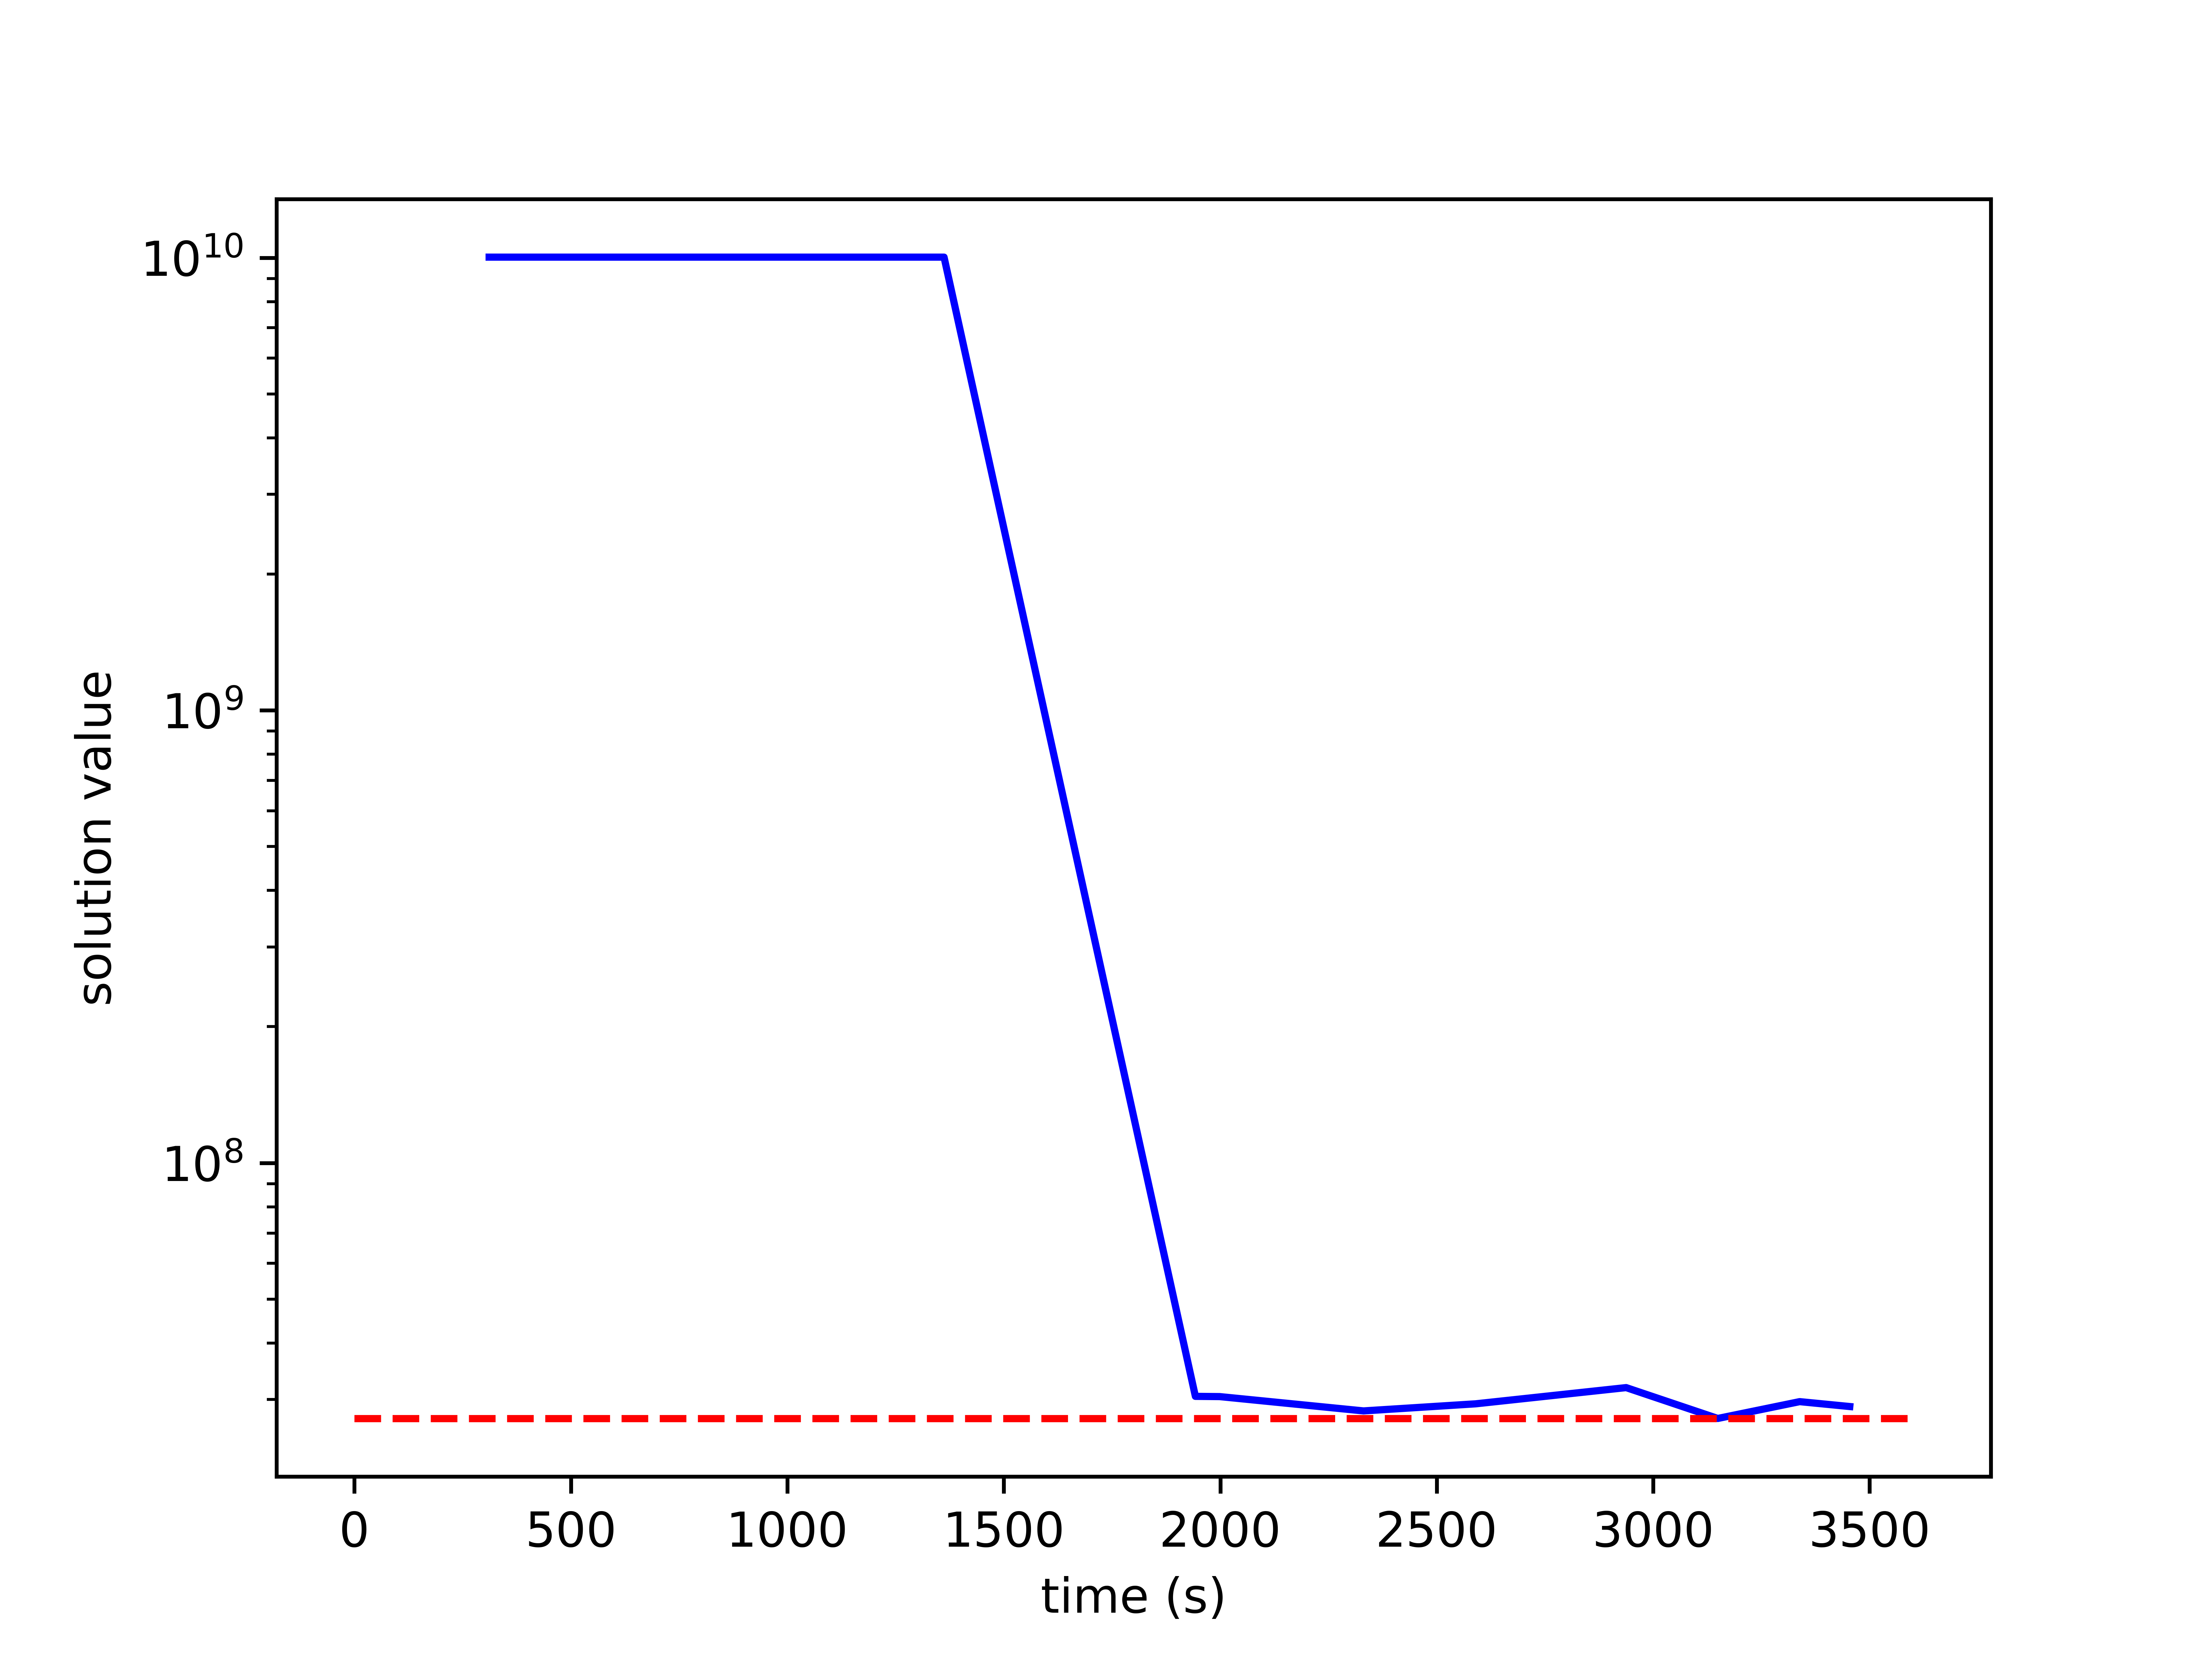
\includegraphics[width=.98\textwidth]{img/perf_plot_VNS_03.png}
\caption{Intermediate values found by the VNS algorithm for instance 3 with a 3600 seconds time limit.}
\label{img:PerfPlotVNS03}
\end{figure}

\begin{figure}[H]
\centering
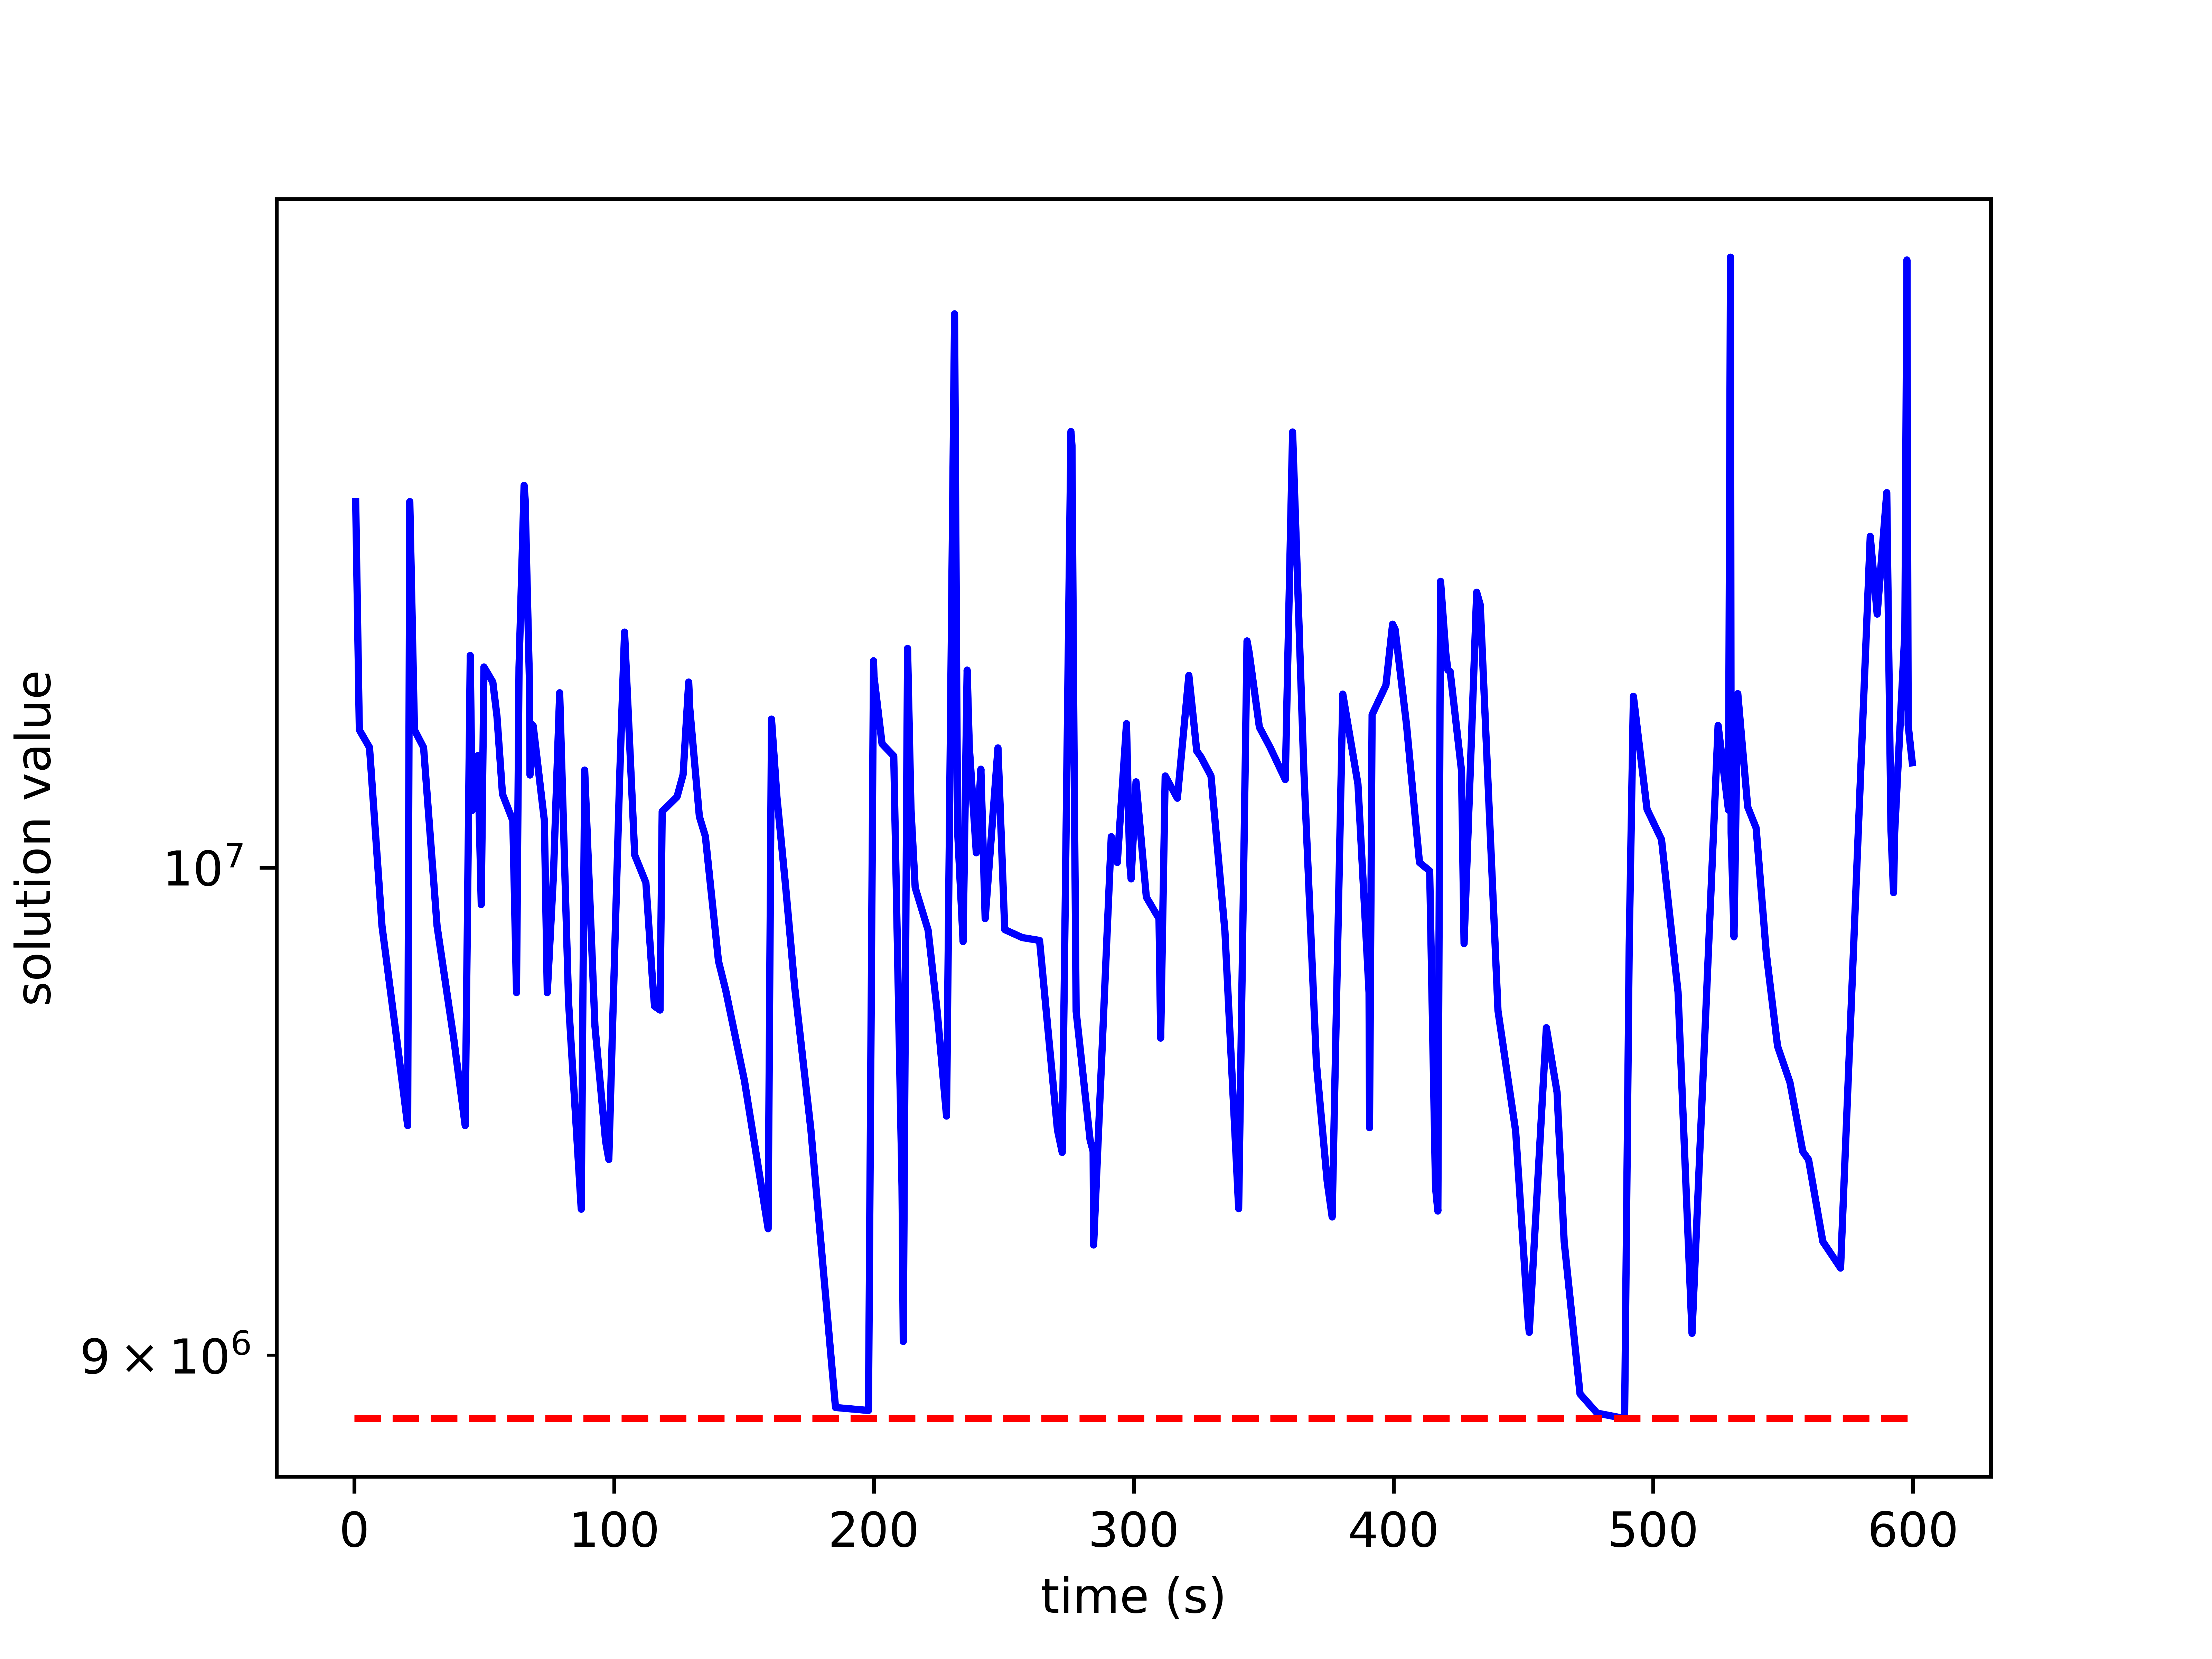
\includegraphics[width=.98\textwidth]{img/perf_plot_VNS_08.png}
\caption{Intermediate values found by the VNS algorithm for instance 8 with a 600 seconds time limit.}
\label{img:PerfPlotVNS08}
\end{figure}


\begin{figure}[H]
\centering
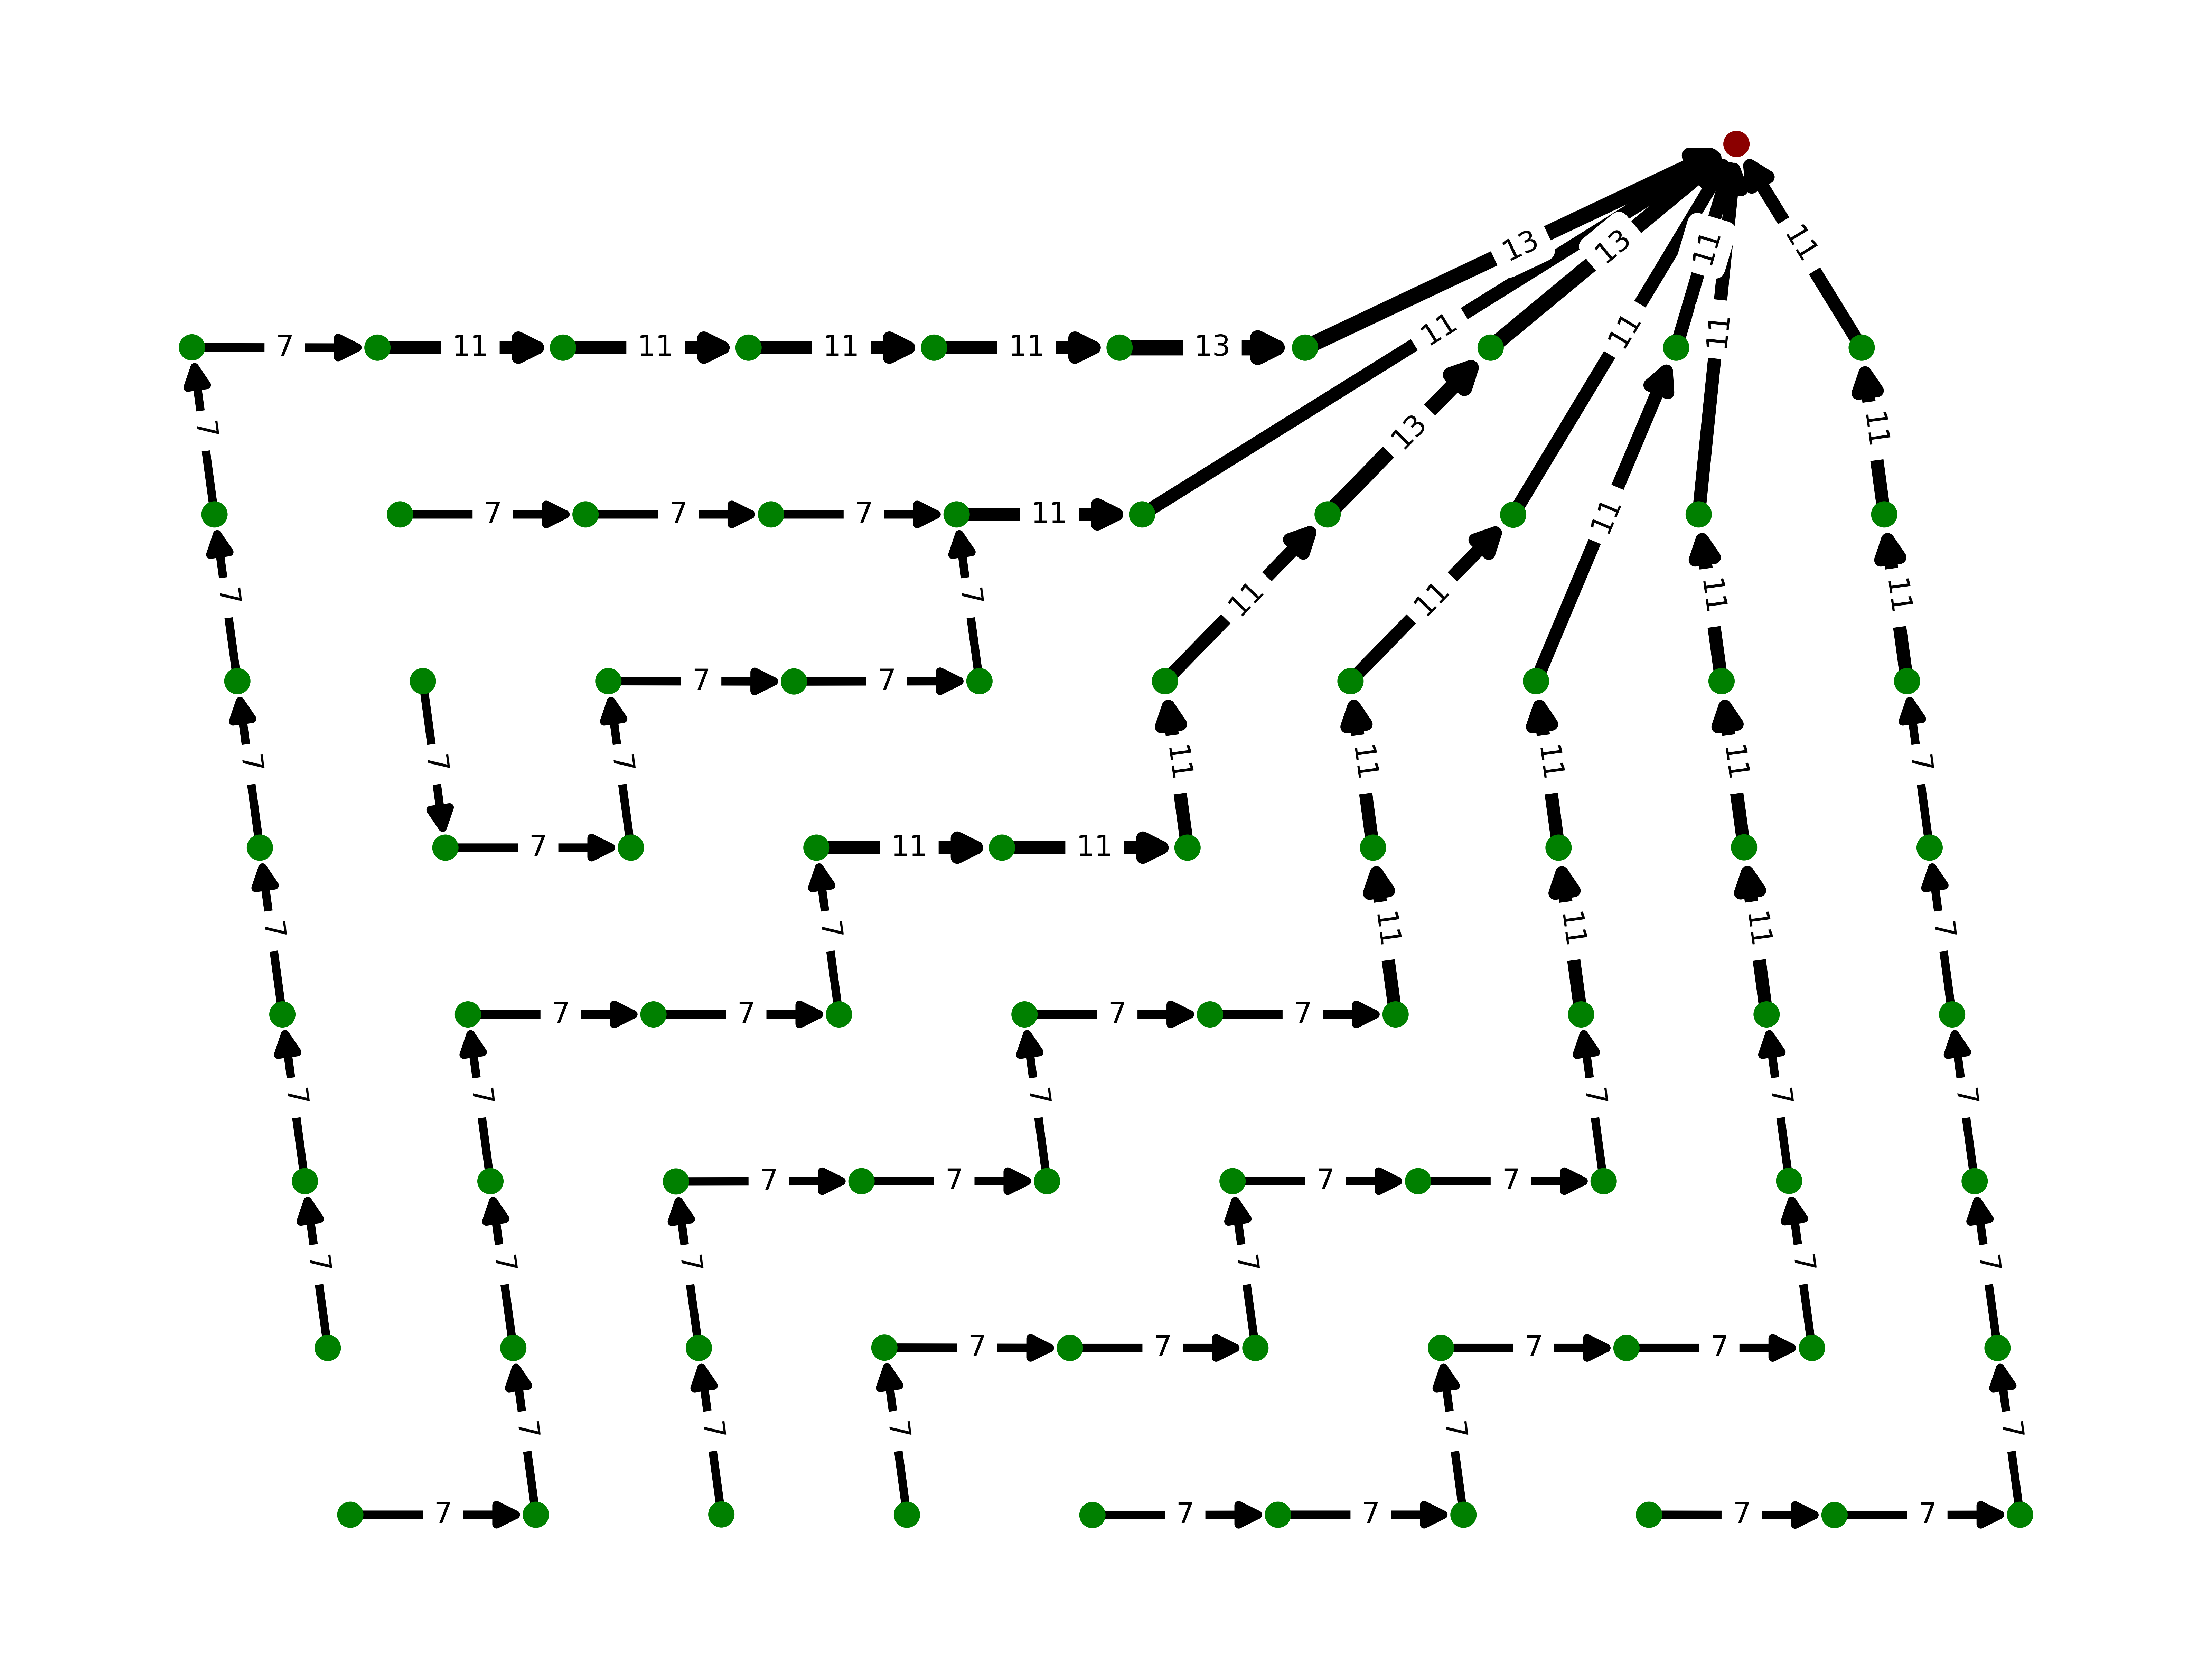
\includegraphics[width=.98\textwidth]{img/hardfix_01_p03.png}
\caption{Final layout for instance 1 obtained with \emph{Hard-fixing} ($p=0.3, t=30\,s$).}
\label{img:Layout01Hardfix_p03}
\end{figure}

\begin{figure}[H]
\centering
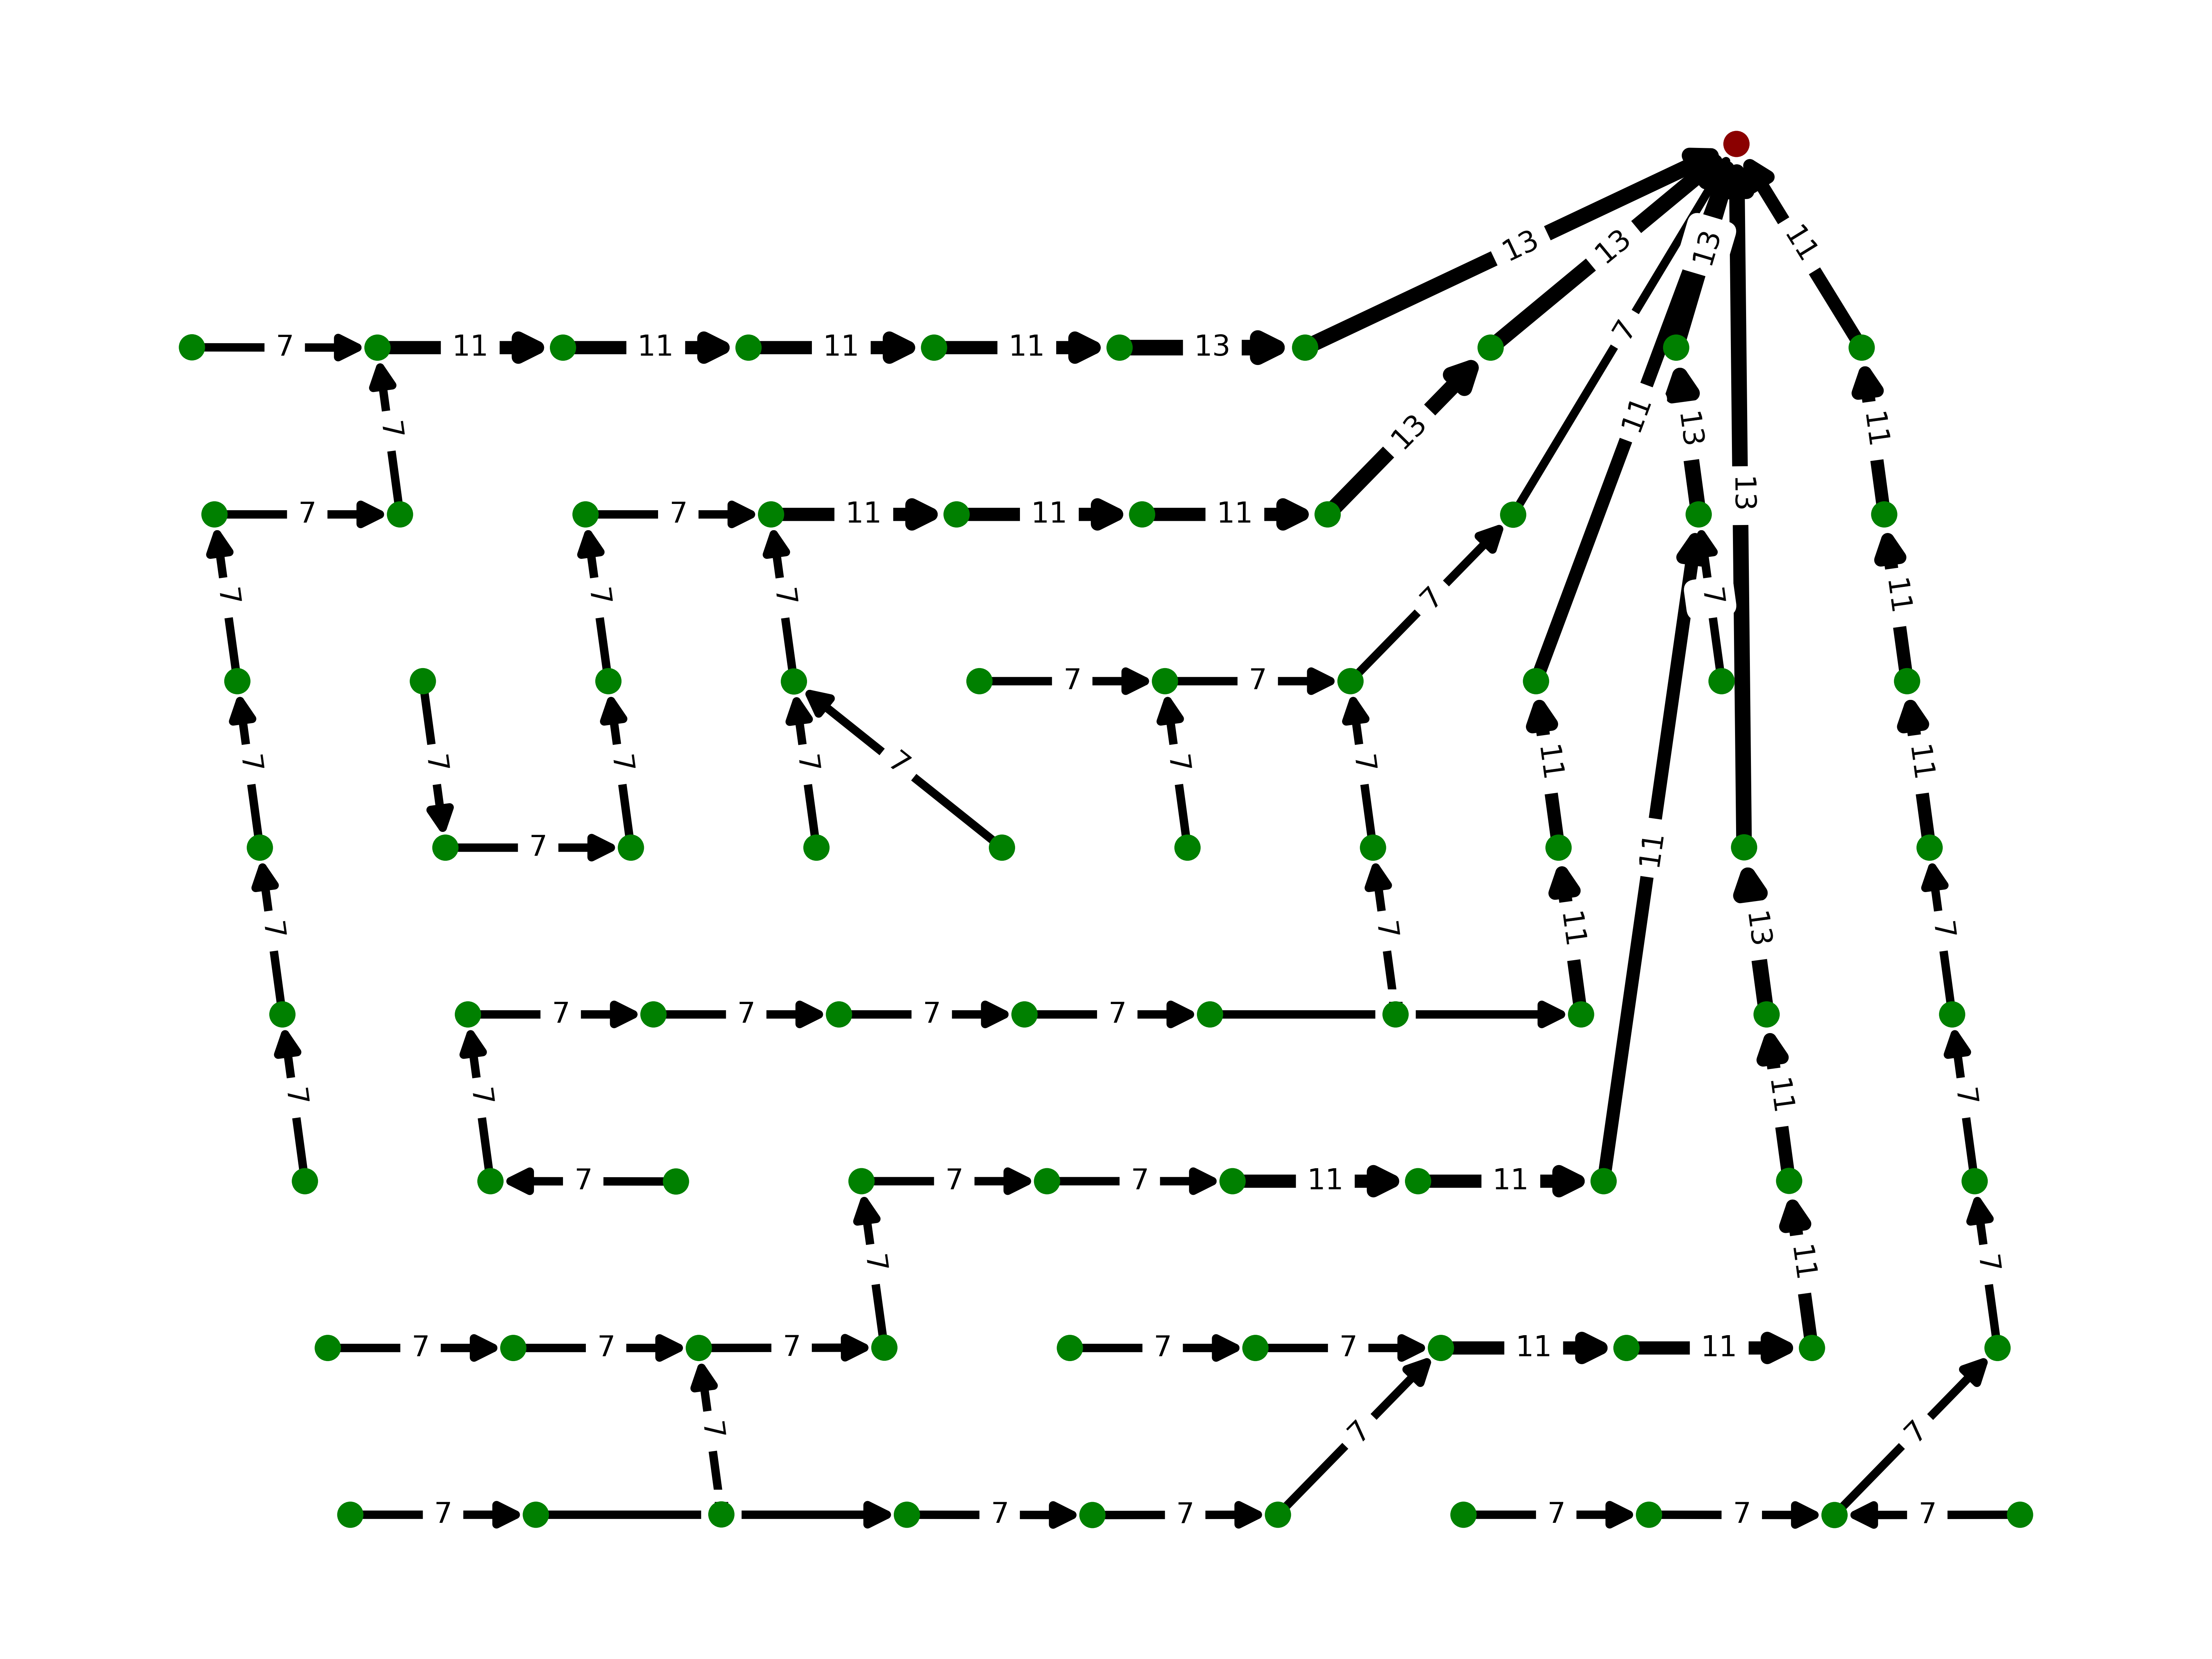
\includegraphics[width=.98\textwidth]{img/hardfix_01_p07.png}
\caption{Final layout for instance 1 obtained with \emph{Hard-fixing} ($p=0.7, t=30\,s$).}
\label{img:Layout01Hardfix_p07}
\end{figure}

\begin{figure}[H]
\centering
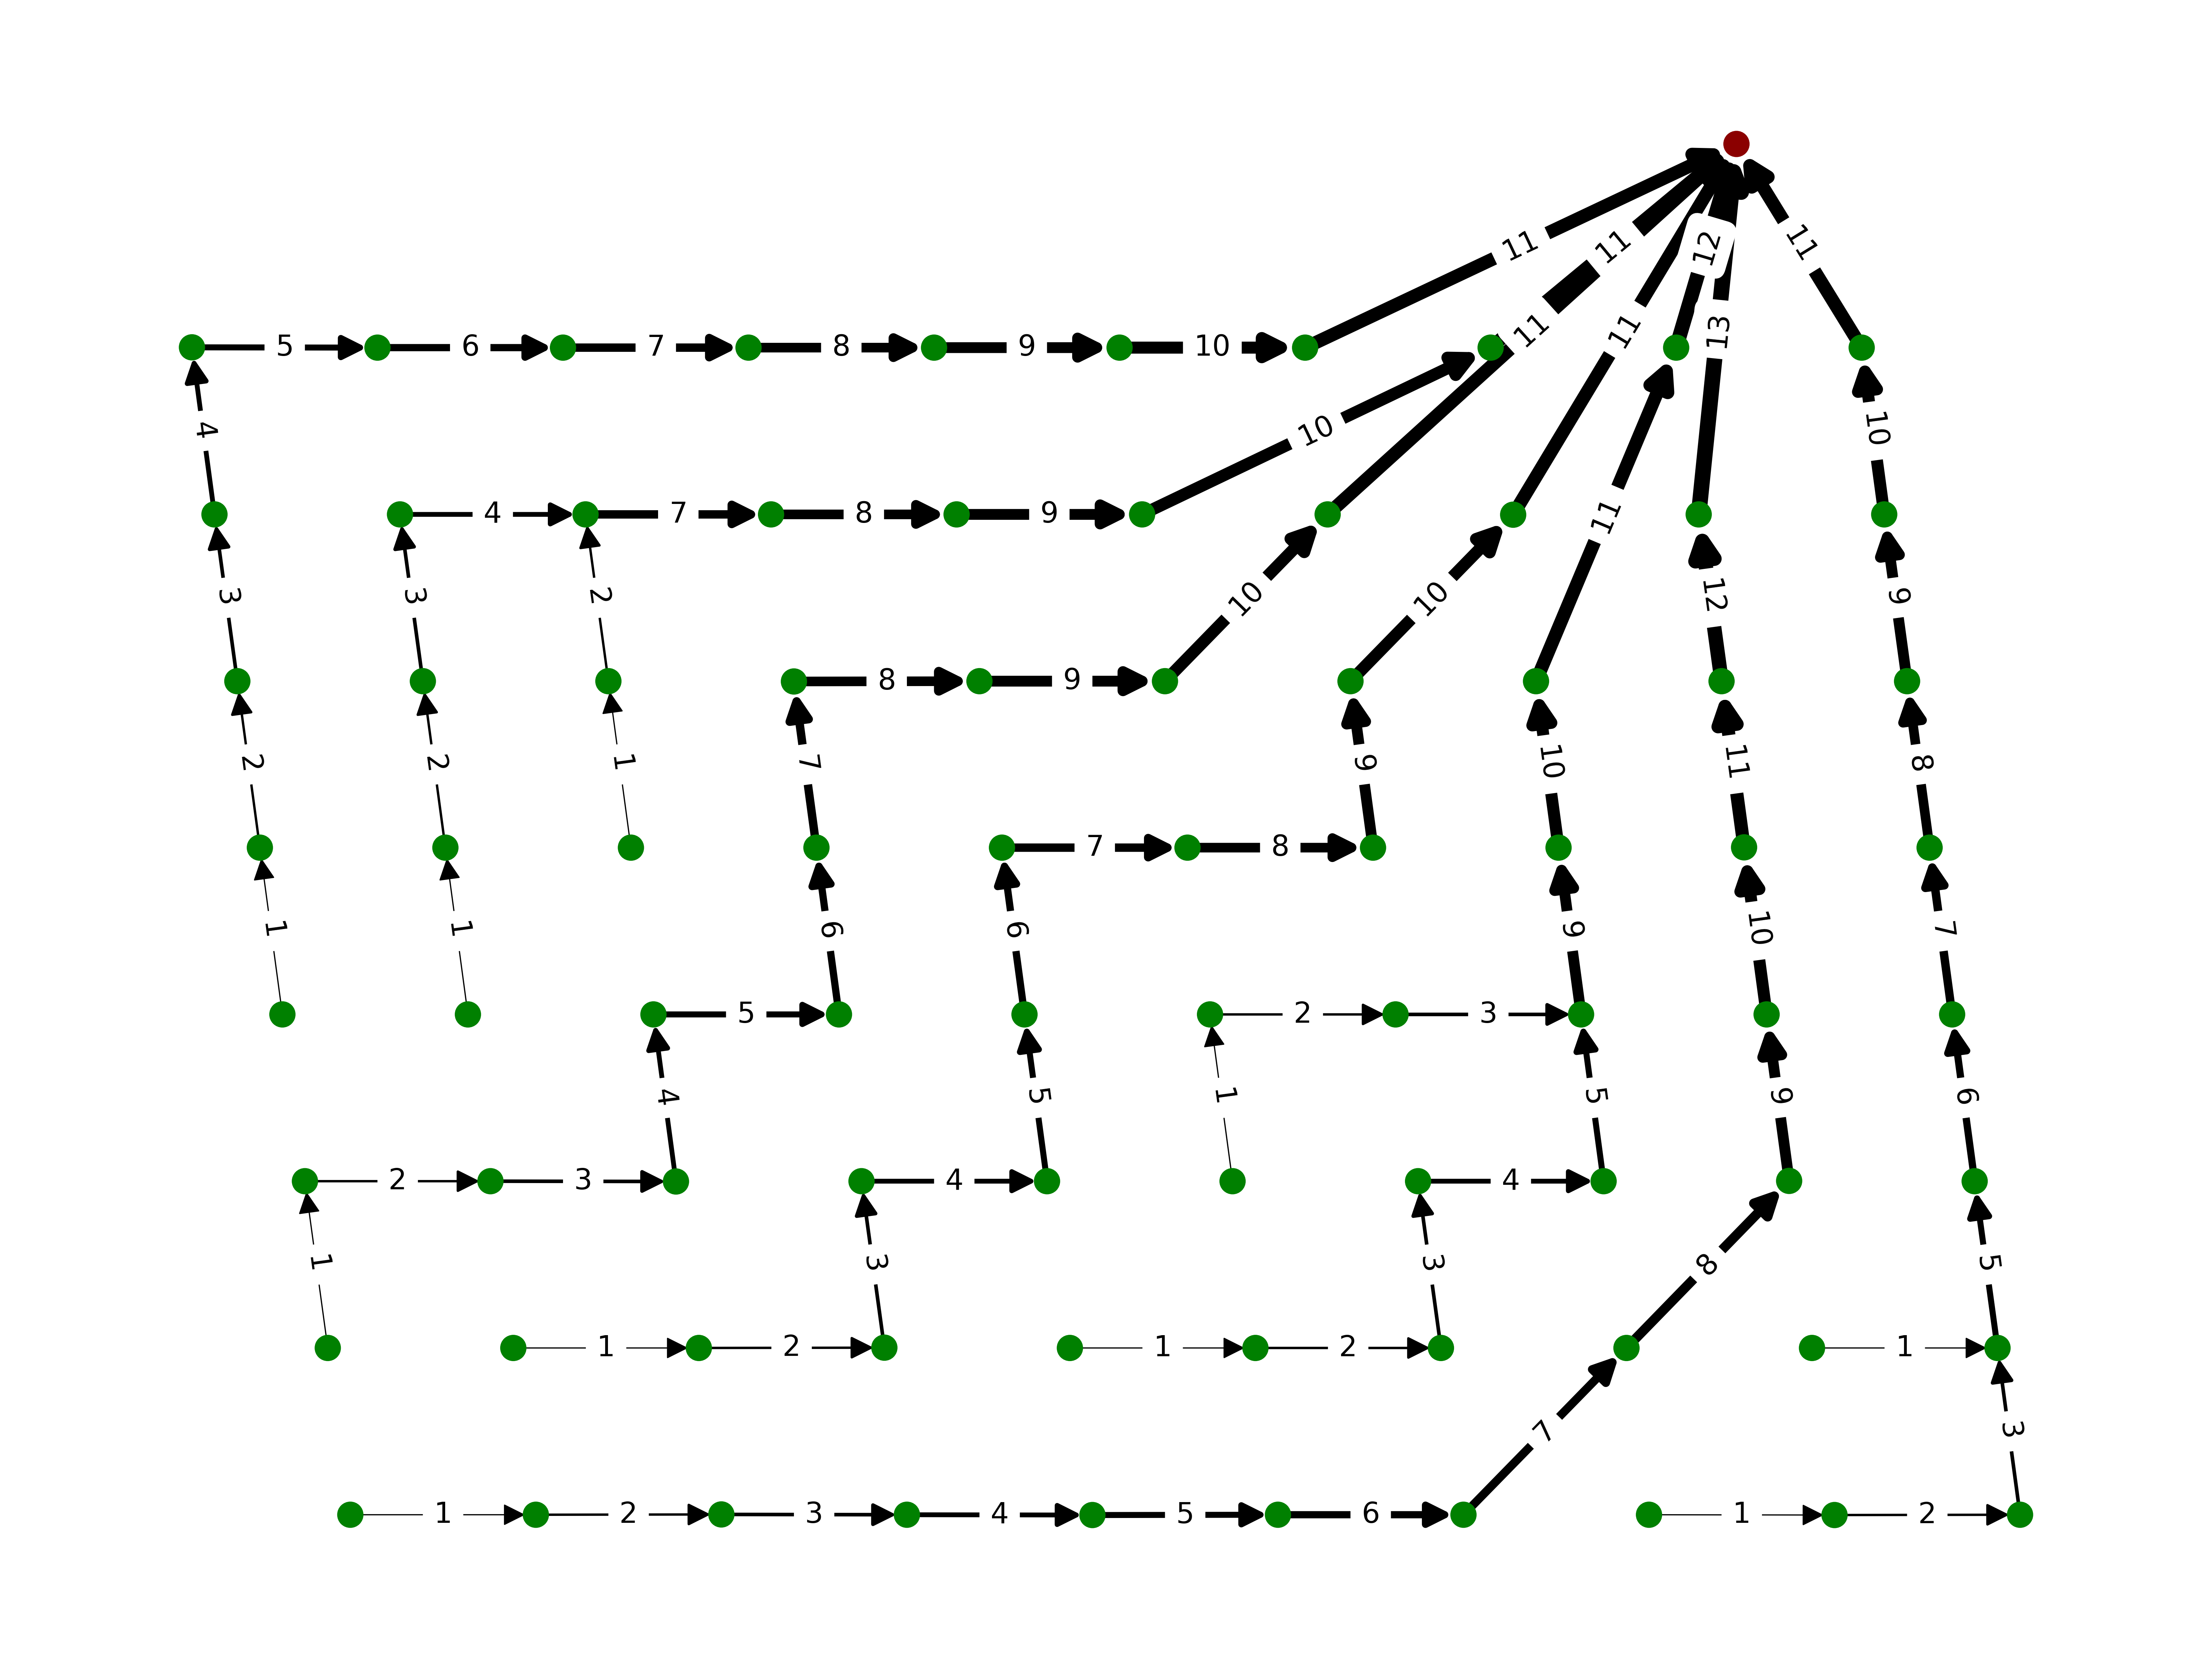
\includegraphics[width=.98\textwidth]{img/hardfix_02_p03.png}
\caption{Final layout for instance 2 obtained with \emph{Hard-fixing} ($p=0.3, t=30\,s$).}
\label{img:Layout02Hardfix_p03}
\end{figure}

\begin{figure}[H]
\centering
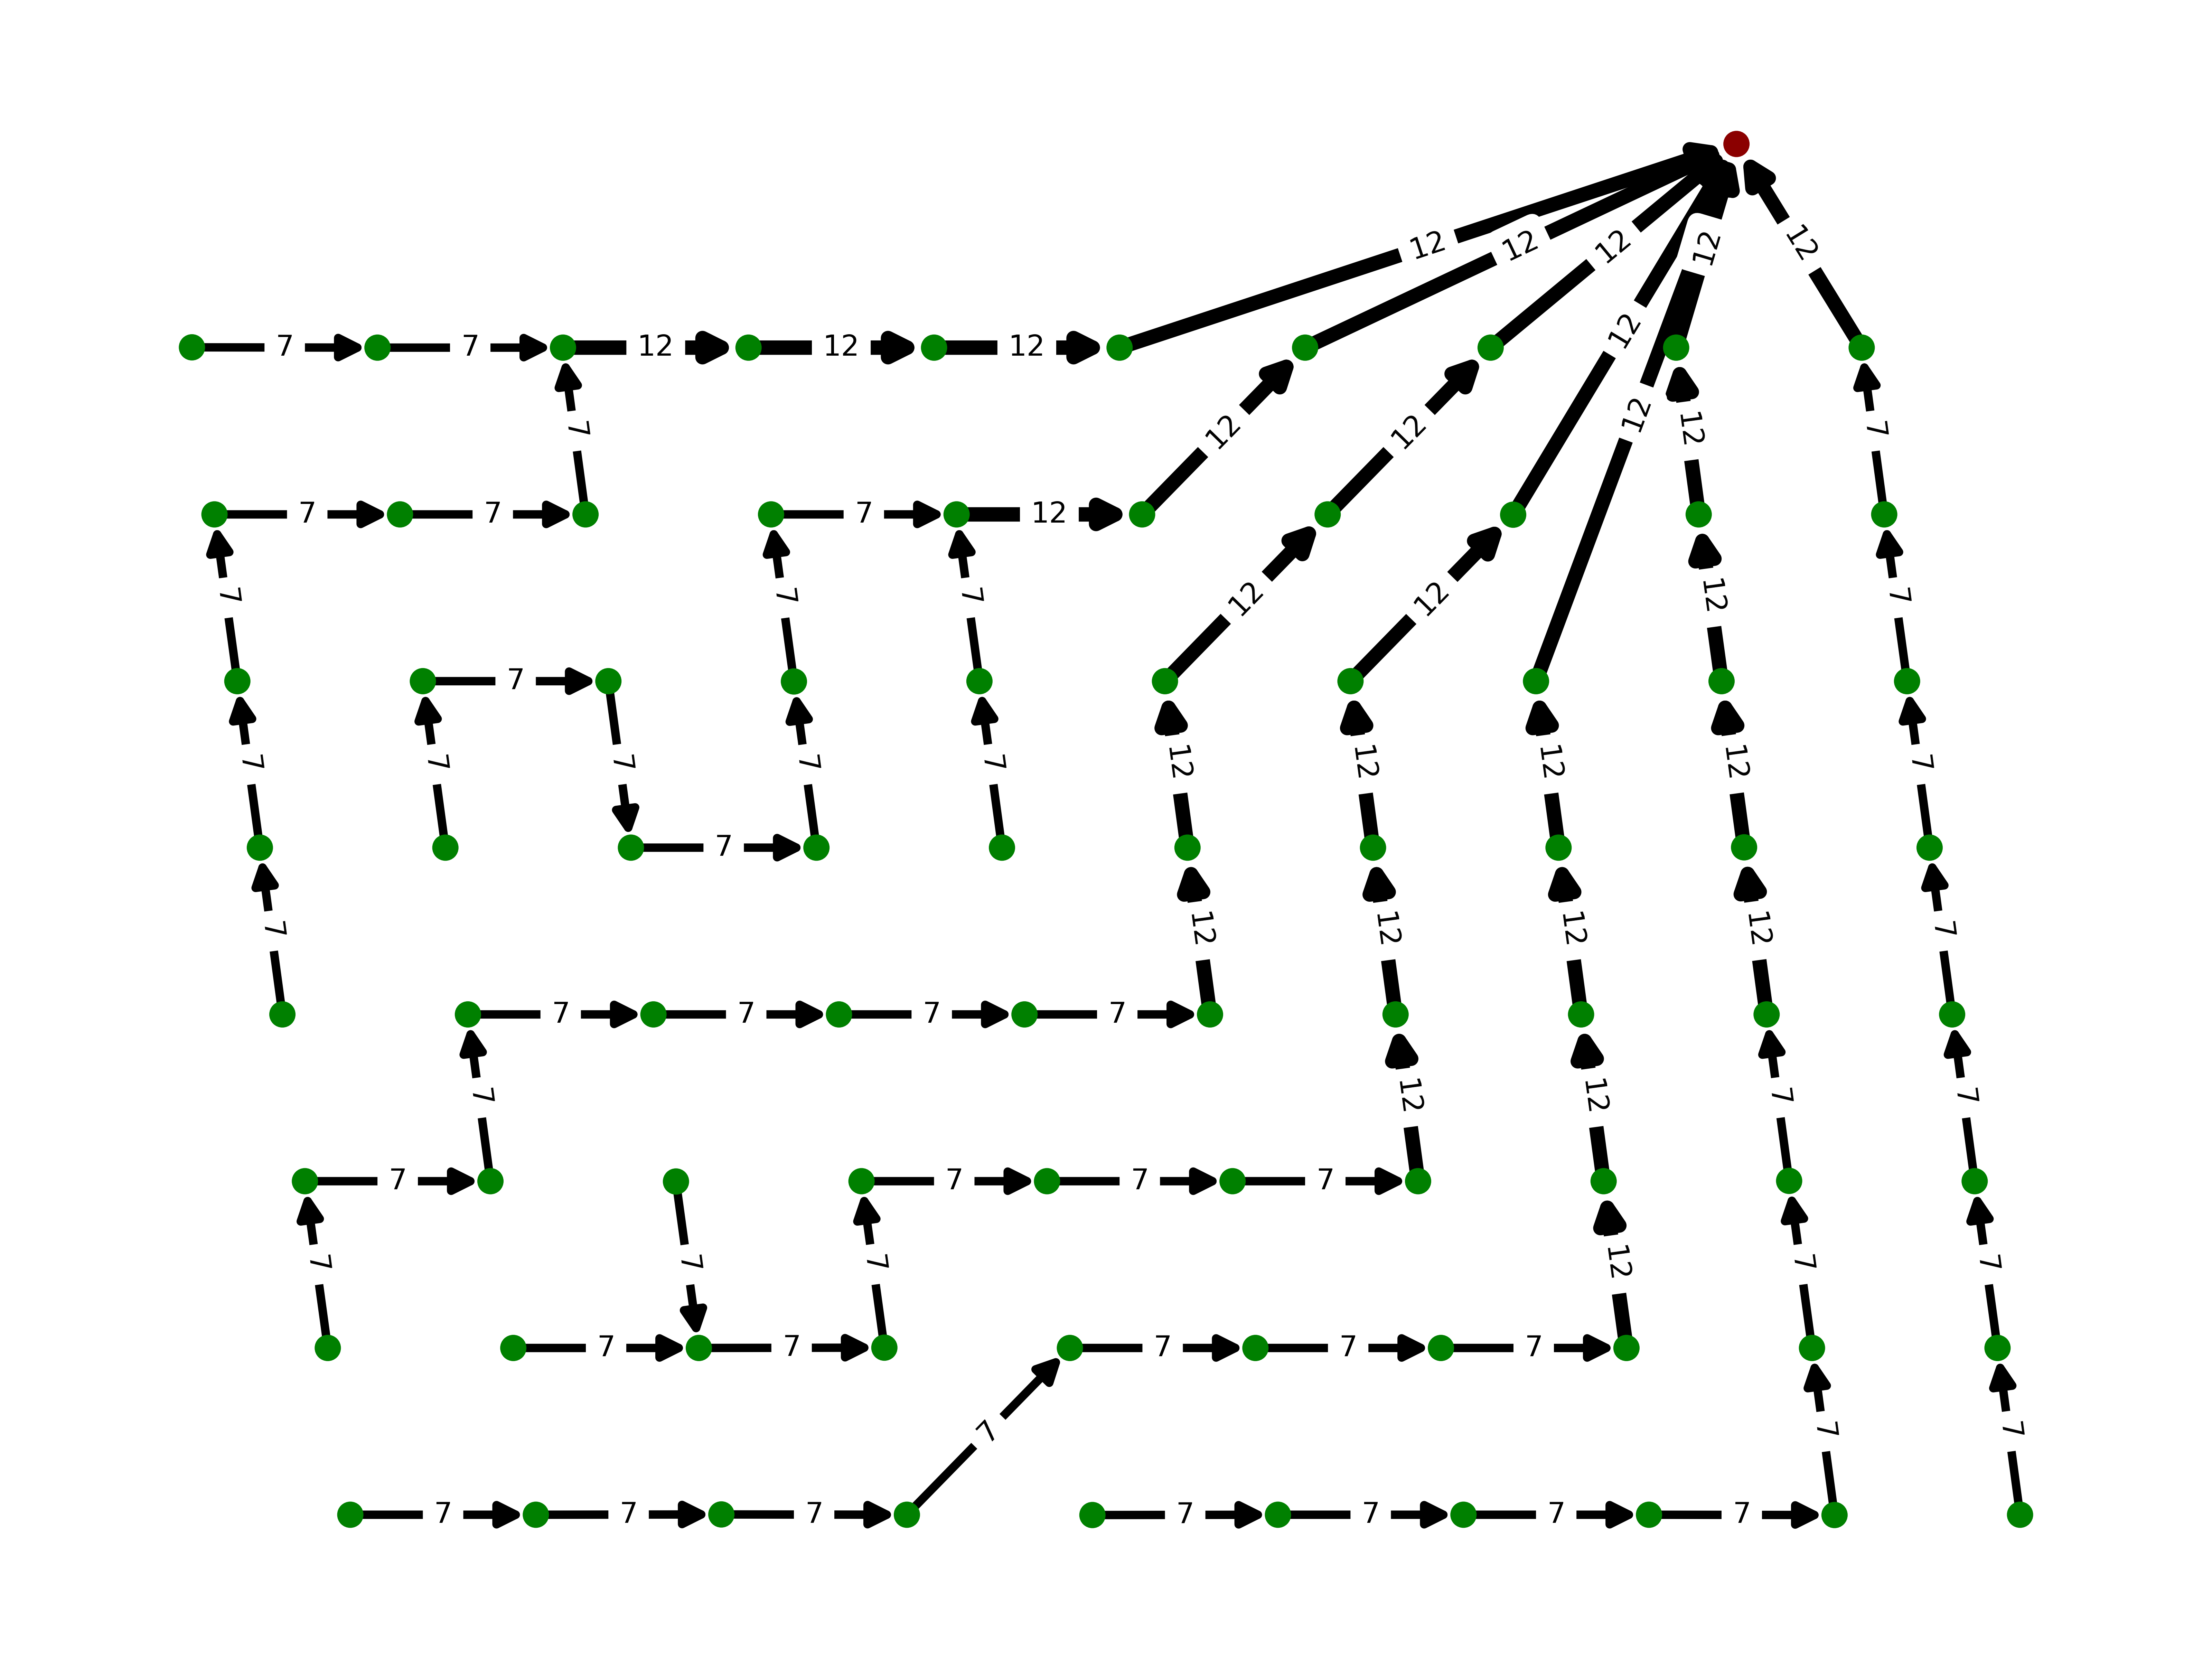
\includegraphics[width=.98\textwidth]{img/hardfix_03_p03.png}
\caption{Final layout for instance 3 obtained with \emph{Hard-fixing} ($p=0.3, t=30\,s$).}
\label{img:Layout03Hardfix_p03}
\end{figure}

\begin{figure}[H]
\centering
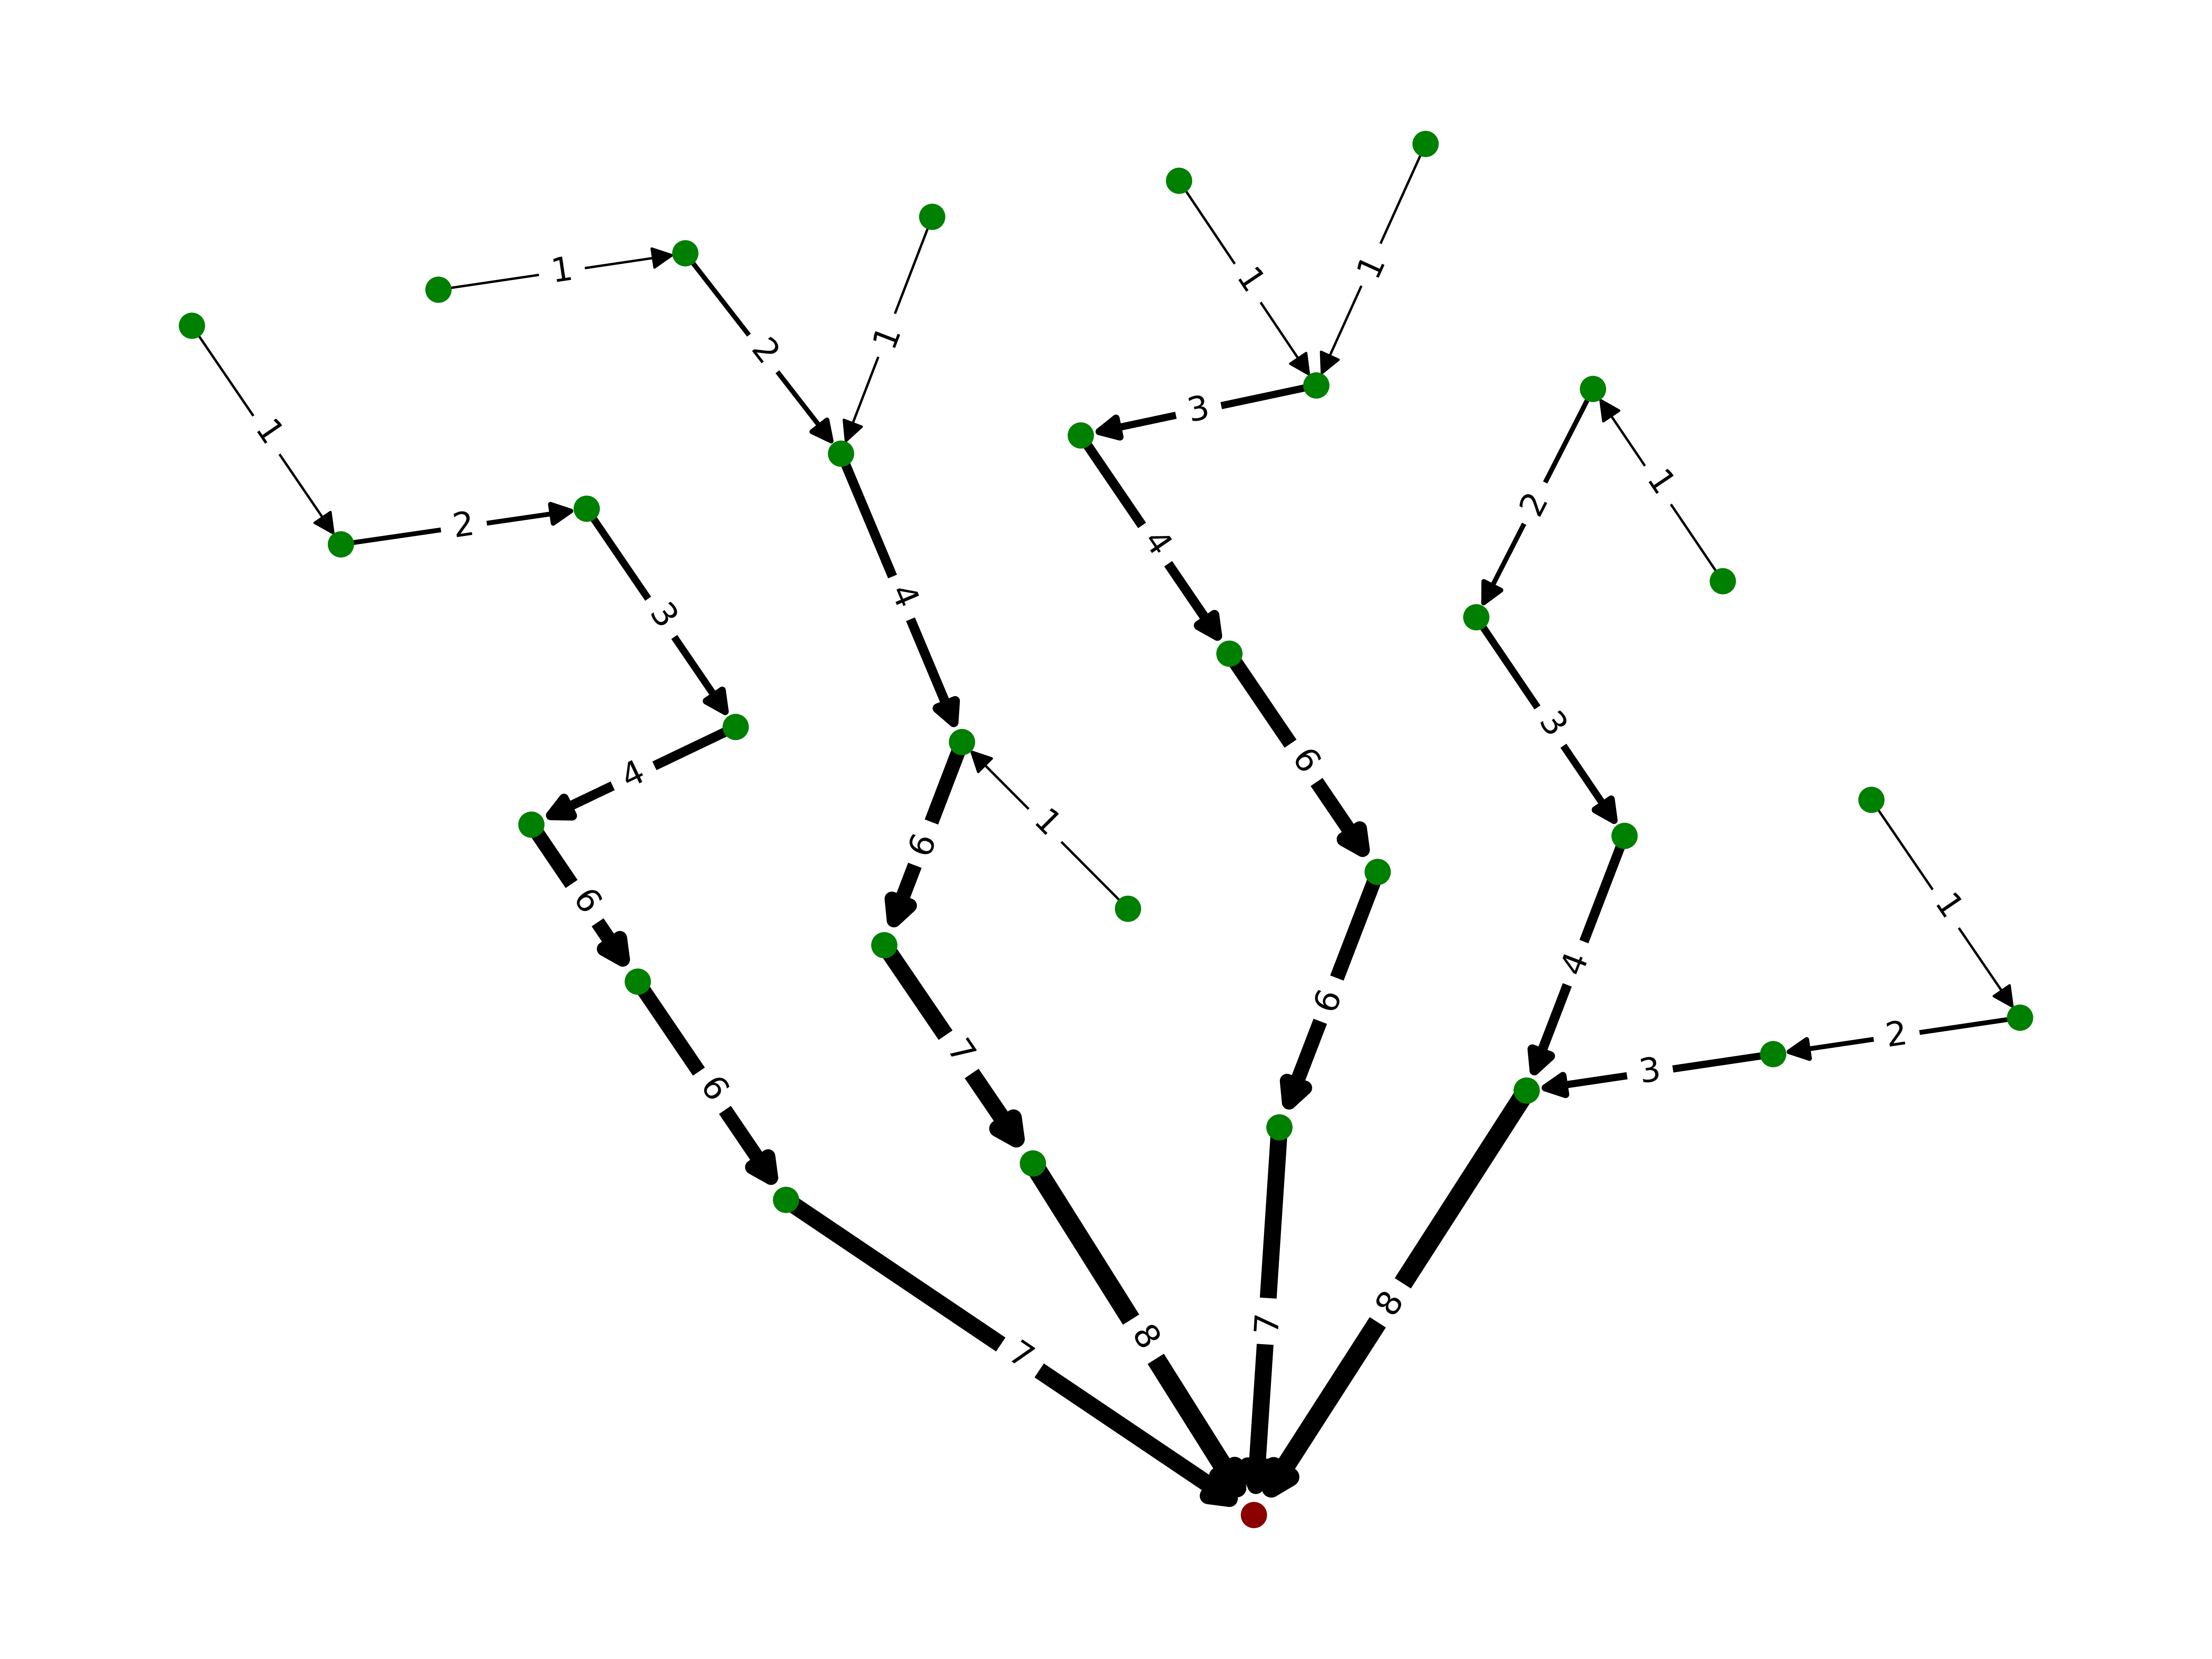
\includegraphics[width=.98\textwidth]{img/hardfix_10_p03.png}
\caption{Final layout for instance 10 obtained with \emph{Hard-fixing} ($p=0.3, t=30\,s$).}
\label{img:Layout10Hardfix_p03}
\end{figure}

\begin{figure}[H]
\centering
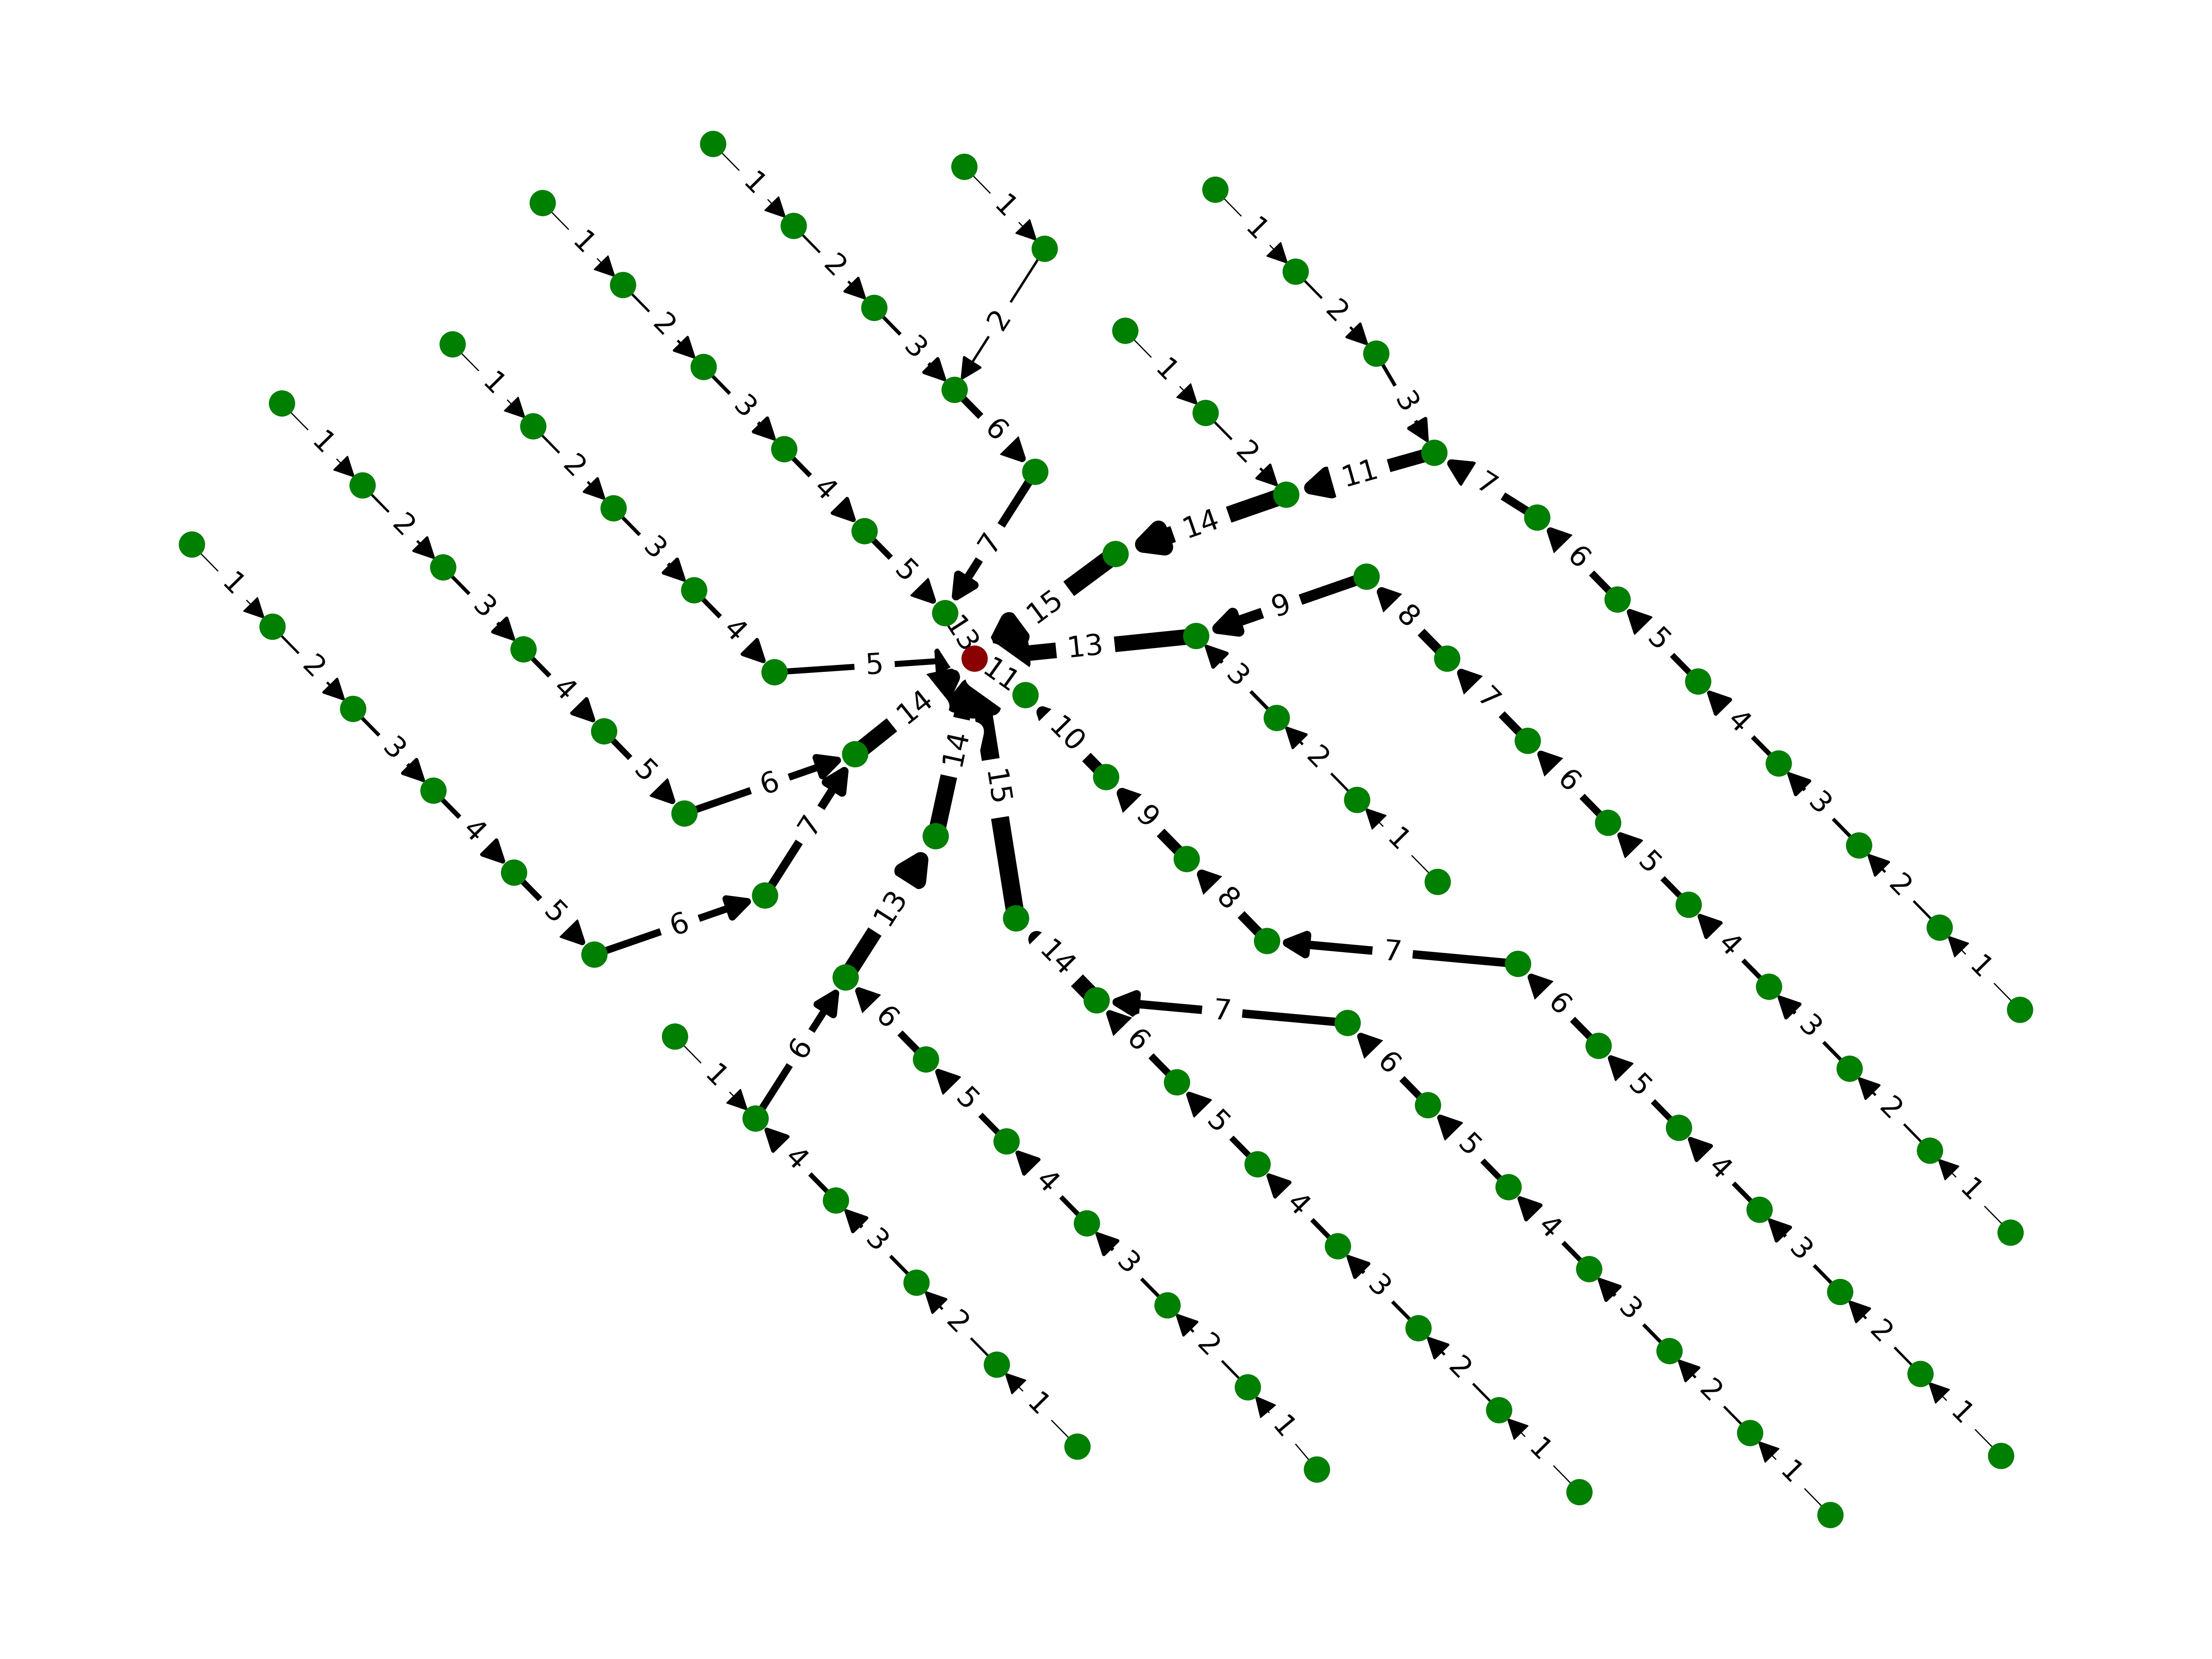
\includegraphics[width=.98\textwidth]{img/hardfix_27_p03.png}
\caption{Final layout for instance 27 obtained with \emph{Hard-fixing} ($p=0.3, t=30\,s$).}
\label{img:Layout27Hardfix_p03}
\end{figure}


\newpage
\section{Conclusions}


%Thanks to this project we were able to discovery the principal difficulties in developing a real optimization project.  

%If heuristics could be a feasible approach with small problems, the use of an expensive solver is well justified when dealing with problems counting hundreds of thousand variables or more. Now the question is: which is a small problem? experience will tell you that 30 turbines are manageable with a heuristic solver.

This project allowed us to engage with common issues in the practical optimization field: from the comprehension and the evaluation of a mathematical model to the implementation of integer programming techniques.

The first approach with \texttt{CPLEX} was rather challenging, nevertheless, we shortly developed the abilities and tools to ensure that the programs we were writing acted as we expected from the theory.

Once we had reached a high level of knowledge about the problem that we were attempting to solve, we have dealt with the development of heuristic algorithms.
Such an approach has conferred us a larger amount of freedom but also more responsibilities. Indeed, it was easier to produce new ideas, yet we ultimately came to realize that many of these were wrong.\\

Moreover, we discovered how a solver can impact in a real-world project in terms of cost saving and how complex it is to achieve similar results by way of implementing specific algorithms for the task.

We think that one of the main purposes of this course is to acquire a deeper critical view of software development in optimization.
By merely studying the theoretical aspects of the discipline, one cannot state which is a \emph{large} instance, and how much time is required to produce an optimal solution, or whether an approach is suitable for a given instance.



\newpage
\section*{Appendix A}
\addcontentsline{toc}{section}{Appendix A}


\subsection*{Setting CPLEX on Mac OS and Ubuntu}
\addcontentsline{toc}{subsection}{Setting CPLEX on OS X and Ubuntu}

Here we provide a procedure for installing the \texttt{IBM ILOG CPLEX Optimization Studio} software on a Mac OS or a Ubuntu machine.

The \texttt{CPLEX} installer is distributed as a \emph{.bin} file and it can be easily downloaded from \url{https://www.ibm.com/it-it/marketplace/ibm-ilog-cplex}.
Students and academics can easily obtain a full version of the product, on the other cases, only a demo version is available.

In order to configure \texttt{CPLEX} on a Mac OS machine, we first have to assign the right permission to execute the installation file. We can make it with the command
\begin{lstlisting}[style=C]
chmod u+x CPLEX_OPT_STUD_[version]_FOR_OSX.bin
\end{lstlisting}

Then we can install the software running
\begin{lstlisting}[style=C]
./CPLEX_OPT_STUD_[version]_FOR_OSX.bin
\end{lstlisting}

The procedure is quite similar for Ubuntu machines. It should look like as the following
\begin{lstlisting}[style=C]
chmod u+x cplex_studio[version].linux-x86.bin 
./cplex_studio[version].linux-x86.bin
\end{lstlisting}

%Once the installation is terminated, we can create a link in %order to run CPLEX from any location.
%This is very practical and we can do it by running
%\begin{lstlisting}[style=C]
%sudo ln -s /Users/USERNAME/Applications/IBM/ILOG/CPLEX_Studio[version]
%/cplex/bin/x86-64_osx/cplex/usr/bin/cplex
%\end{lstlisting}

To be certain the installation is correctly accomplished, we can run some examples, such as 
\begin{lstlisting}[style=C]
cd /CPLEX_BASE_DIR/examples/SYSTEM/static_pic
make ilolpex1
./ilolpex1 -r
\end{lstlisting}

By using \texttt{CPLEX} with the C language, as we did, it is necessary to tell the compiler how to find the \emph{include} directory and to specify the linker where is the library location.
With the \texttt{gcc} compiler, this should look like as
\begin{lstlisting}[style=C]
gcc -I/CPLEX_BASE_DIR/include/ilcplex -L/CPLEX_BASE_DIR/lib/x86-64_[SYSTEM]/static_pic -lcplex -lm -lpthread -ldl
\end{lstlisting}
To conclude, it shouldn't forget to add this line to the file in which \texttt{CPLEX} functions are called
\begin{lstlisting}[style=C]
#include <cplex.h>
\end{lstlisting}

\newpage

\bibliographystyle{plain}
\bibliography{Report}

\end{document}
